\documentclass[utf8,german,beleg]{zihpub}

\usepackage{caption}
\usepackage{datetime}
\usepackage{etoolbox}
\usepackage[acronyms,nonumberlist,toc,xindy]{glossaries}
\usepackage[chapter,newfloat]{minted}
\usepackage{tcolorbox}
\usepackage{tikz}

\newenvironment{code}{\captionsetup{type=listing}}{}
\SetupFloatingEnvironment{listing}{name=Quelltext}

\usetikzlibrary{arrows}

\BeforeBeginEnvironment{minted}{\begin{tcolorbox}}
\AfterEndEnvironment{minted}{\end{tcolorbox}}

\newcommand{\lstfont}[1]{\color{#1}\small\ttfamily}

\definecolor{keyword-green}{RGB}{0, 128, 0}

\author{Jan Stephan}
\title{Untersuchung der Parallelisierung des Feldkamp-Davis-Kress-Algorithmus mittels CUDA{\textregistered}}
\matno{3755136}
\betreuer{\hspace{0.15mm}Dr.-Ing. André Bieberle \\
          \qquad \qquad Dr.-Ing. Guido Juckeland \\
          \qquad \qquad Matthias Werner}
\date{21. März 2017}
\copyrighterklaerung{Ich habe wirklich nichts geklaut}
\acknowledgments{Für die fachliche Betreuung bei der Erstellung dieser Arbeit bedanke ich mich recht herzlich bei Herrn
                 Dr.-Ing.\ Stephan Boden von der AREVA-Stiftungsprofessur für bildgebende Messverfahren für die
                 Energie- und Verfahrenstechnik.}
\bibfiles{bibliography.bib}

\makeglossaries
\newglossaryentry{kernel}{name=Kernel,
                          description={Programm, das auf einem Beschleuniger, wie etwa einer GPU, ausgeführt wird},
                          plural=Kernel}
\newglossaryentry{cuda}{name={CUDA{\textregistered}},
                        description={NVIDIA{\textregistered} CUDA{\textregistered},
                                     proprietäre Plattform für die Programmierung von Grafikkarten}}
\newglossaryentry{directx}{name={DirectX{\textregistered}},
                           description={Microsoft{\textregistered} DirectX{\textregistered},
                                        proprietäre Plattform für u.a. Grafikprogrammierung}}
\newglossaryentry{pixel}{name=Pixel,
                         description={Punkt in einem zweidimensionalen Koordinatensystem, z.B.\ einem Bild oder einem
                                      Detektor},
                         plural=Pixel}
\newglossaryentry{voxel}{name=Voxel,
                         description={Punkt in einem dreidimensionalen Koordinatensystem, z.B.\ einem Volumen},
                         plural=Voxel}
\newglossaryentry{host}{name=Host,
                        description={Gerät, das einen Kernel auf dem Device ausführt. Üblicherweise ist dies das Gerät,
                                     auf dem auch das Betriebssystem läuft, etwa ein Rechner oder ein Knoten auf einem
                                     Superrechner},
                        plural=Hosts}
\newglossaryentry{device}{name=Device,
                          description={Beschleuniger, der einen Kernel ausführt. Im Zusammenhang mit
                                       CUDA{\textregistered} ist dieser typischerweise eine GPU},
                          plural=Devices}
\newglossaryentry{stream}{name=Stream,
                          description={Warteschlange auf einem \gls{cuda}-\gls{device}. Operationen, wie z.B.\
                                       \gls{kernel}aufrufe, werden innerhalb eines Streams sequentiell ausgeführt.
                                       Mehrere Streams können vom gleichen \gls{device} parallel abgearbeitet werden},
                          plural=Streams}

\newacronym{fdk}{FDK-Algorithmus}{Feldkamp-Davis-Kress-Algorithmus}
\newacronym{hzdr}{HZDR}{Helmholtz-Zentrum Dresden-Rossendorf}
\newacronym{paris}{PARIS}{\textit{Portable and Accelerated 3D Reconstruction tool for radiation based Imaging
                                  Systems}}
\newacronym{fpga}{FPGA}{\textit{Field Programmable Gate Array}}
\newacronym{opencl}{OpenCL{\texttrademark}}{\textit{Open Computing Language}}
\newacronym{fpu}{FPU}{\textit{floating point unit}}
\newacronym{gpgpu}{GPGPU}{\textit{General Purpose Computation on Graphics Processing Unit}}
\newacronym{opengl}{OpenGL{\texttrademark}}{\textit{Open Graphics Library}}
\newacronym{openmp}{OpenMP{\textregistered}}{\textit{Open Multi-Processing}}
\newacronym{openacc}{OpenACC{\textregistered}}{\textit{Open Accelerators}}
\newacronym{gpu}{GPU}{\textit{Graphics Processing Unit}}
\newacronym{cpu}{CPU}{\textit{Central Processing Unit}}
\newacronym{simd}{SIMD}{\textit{Single Instruction, Multiple Data}}
\newacronym{simt}{SIMT}{\textit{Single Instruction, Multiple Threads}}
\newacronym{sm}{SM}{\textit{Streaming Multiprocessor}}
\newacronym{gpc}{GPC}{\textit{Graphics Processing Cluster}}

% Germanisiere LaTeX
\deftranslation[to=German]{Acronyms}{Abkürzungsverzeichnis}
\deftranslation[to=German]{Glossary}{Glossar}
\renewcommand*{\listlistingname}{Quelltextverzeichnis}

\begin{document}

\printglossaries
\listoffigures
\listoflistings
\listoftables

\chapter{Einleitung}

\section{Die Geschichte und Relevanz der Computertomographie}

Die Geschichte der Computertomographie beginnt mit dem vom deutschen Physiker Wilhelm Conrad Röntgen entdeckten
und später nach ihm benannten Verfahren der {\glqq}X-Strahlen{\grqq} (vgl.~\cite{roentgen}). Plötzlich war es möglich,
die innere Beschaffenheit eines Objekts auf nichtinvasive Art und Weise zu untersuchen. Die Bedeutung dieses Verfahrens
insbesondere für die Anwendung in der Medizin war bereits Röntgens Zeitgenossen klar. So druckte die Wiener Zeitung
{\glqq}Die Presse{\grqq} am 05.\ Januar 1896 auf ihrer Titelseite unter der Überschrift {\glqq}Eine sensationelle
Entdeckung{\grqq}: {\glqq}[Man hat es] mit einem in seiner Art epochemachenden Ergebnisse der exacten Forschung zu thun,
das sowol [sic] auf physikalischem wie auf medicinischem Gebiete ganz merkwürdige Consequenzen bringen dürfte.{\grqq}
Für seine Entdeckung wurde Röntgen in der Folge unter anderem mit dem ersten Nobelpreis für Physik ausgezeichnet.

Führt man eine Röntgenaufnahme (\textit{Vorwärtsprojektion}) genügend oft in aufeinanderfolgenden Winkelschritten aus,
bis man (idealerweise) einen Vollkreis abgefahren hat, so lässt sich aus den dabei entstandenen Abbildungen
(\textit{Projektionen}) der durchleuchtete Körper rekonstruieren (\textit{Rückprojektion}). Diese Vorgehensweise wurde
in den 60er Jahren des 20. Jahrhunderts durch den südafrikanisch-amerikanischen Physiker Allan McLeod Cormack
entwickelt, der ebenfalls die dazu notwendigen mathematischen Grundlagen herleitete (vgl.~\cite{cormack63}
und~\cite{cormack64}). Ihm war allerdings nicht bekannt, dass diese Grundlagen schon 1917 vom österreichischen
Mathematiker Johann Radon gefunden wurden (vgl.~\cite{cormack79}). Mathematisch ist der Vorgang der
\textit{Rückprojektion} die Inversion der nach Radon benannten \textit{Radon-Transformation} (vgl.~\cite{radon}).

Da die Rückprojektion für jeden Punkt im Körper einzeln berechnet werden muss, ist sie für einen Menschen nicht in
sinnvoller Zeit lösbar. Aus diesem Grund ist man für die Lösung des Gesamtproblems auf einen Computer angewiesen, woraus
sich der Name des Verfahrens ableitet: \textit{Computertomographie}. Die ersten bis zur Marktreife entwickelten
Computertomographen wurden gegen Ende der 60er Jahre des 20. Jahrhunderts vom englischen Elektroingenieur Godfrey
Hounsfield gebaut (vgl.~\cite{houns}). Dieser entwickelte die für die Rückprojektion nötigen Algorithmen ebenfalls
selbst, da ihm die Vorarbeiten von Cormack und Radon nicht bekannt waren. Für ihre Arbeiten erhielten Hounsfield und
Cormack 1979 den Nobelpreis für Physiologie oder Medizin, was die Bedeutung der Computertomographie für die Medizin
unterstreicht.

Bis heute ist die Computertomographie ein bedeutendes Verfahren zur nichtinvasiven Analyse von Strukturen innerhalb
eines Körpers. Dabei wird sie nicht nur in der Medizin angewendet, sondern ebenfalls in der Materialforschung
eingesetzt. Für Projektionen, die im dreidimensionalen Raum mit Hilfe eines Kegelstrahls erzeugt wurden, haben Feldkamp,
Davis und Kress 1984 einen Rückprojektionsalgorithmus entwickelt, der einfach zu implementieren ist (vgl.~\cite{fdk}).
Dieser Algorithmus wird im Allgemeinen nach seinen drei Entwicklern \gls{fdk} genannt. Aufgrund des technischen
Fortschritts bei der Geräteentwicklung und Detektorauflösung und der damit zusammenhängenden, stetig wachsenden
Datenmenge ist eine effiziente Implementierung der Rückprojektion auch heute noch wichtig. Eine Möglichkeit zur
schnellen Verarbeitung dieser Datenmenge liegt im Einsatz von Grafikkarten, deren für parallele Berechnungen von
computergrafischen Problemen ausgelegte Architektur für die Rückprojektion große Vorteile verspricht.

\section{Aufgabenstellung}\label{intro:aufgabenstellung}

Das Ziel dieser Arbeit ist, die Parallelisierung des \gls{fdk} mit Grafikkarten zu untersuchen. Zum Einsatz kommt dabei
die vom Grafikkartenhersteller NVIDIA entwickelte \gls{cuda}-Plattform. Da die Verwendung von Grafikkarten mit
Limitierungen verbunden ist, wie etwa einem im Vergleich zu herkömmlichen Prozessoren begrenzten Speicher, sollen die
folgenden Implementierungsziele erreicht werden:

\begin{enumerate}
    \item Der begrenzte Speicher auf der \gls{gpu} soll möglichst effizient genutzt werden. Häufige Kopien zwischen dem
          Hauptspeicher der \gls{cpu} und dem der \gls{gpu} sind also zu vermeiden.
    \item Die Rückprojektion soll die Rechenressourcen der \gls{gpu} möglichst optimal ausnutzen.
    \item Wenn mehrere \gls{gpu}s zur Verfügung stehen, sollen diese auch genutzt werden.
\end{enumerate}

Die Parallelisierung des \gls{fdk} ist seit seiner Vorstellung immer wieder Gegenstand der Forschung gewesen. Die
Umsetzung der vorgenannten Ziele bedingt also zunächst eine Analyse der bisher erfolgten Arbeiten, insbesondere im
Hinblick auf die Verwendung von \gls{gpu}s, sowie einen Variantenvergleich der erfolgsversprechenden Ideen. Aus diesem
ist dann ein Ansatz herzuleiten, dessen Implementierung dann im Hinblick auf die Zielstellung analysiert wird.

\chapter{Grundlagen}\label{chap:grundlagen}

Dieses Kapitel stellt das theoretische Fundament der späteren praktischen Arbeit vor. Zunächst werden die
mathematischen und algorithmischen Grundlagen der Computertomographie erläutert, bevor die \gls{cuda}-Plattform als
technische Basis eingeführt wird.

\section{Die Computertomographie}

\subsection{Mathematische Grundlagen der Computertomographie}

In diesem Abschnitt werden die mathematischen Grundlagen der Computertomographie behandelt. Es werden zunächst die
mathematischen Eigenschaften der Vorwärtsprojektion und das sich daraus ergebende Fourier-Schichten-Theorem erläutert.
Anschließend wird die Aufnahme der Projektionen mit Parallelstrahlen erklärt und die Aufnahme mit Fächerstrahlen
abgeleitet. Zum Schluss wird das Prinzip der Fächerstrahlen auf den dreidimensionalen Raum ausgeweitet, also auf die
Aufnahme mit Kegelstrahlen.

\subsubsection{Projektionen}

Schießt man einen Röntgenstrahl durch ein festes Objekt, wie beispielsweise biologisches Gewebe oder ein Metall, so wird
dieser Strahl je nach Dichte des Materials entlang seiner Bahn abgeschwächt bzw.\ absorbiert. Mathematisch lässt sich
ein Objekt als zwei- oder dreidimensionale Verteilung von Absorptionskonstanten verstehen, während die gesamte
Abschwächung entlang einer Strahlbahn als Kurvenintegral dargestellt werden kann.

Die Grundlage der folgenden Ausführungen ist die Abbildung~\ref{fig:math_proj}~\cite{kak}. Als Beispiel dienen ein
Objekt, dargestellt als die Funktion $f(x, y)$, sowie Kurvenintegrale, dargestellt durch das Parameterpaar
$(\alpha, t)$. Die Linie $AB$ lässt sich dann durch die folgende Formel darstellen:

\begin{equation*}
    x \cdot \cos \alpha + y \cdot \sin \alpha  = t_1
\end{equation*}

oder allgemein für beliebige, zu $AB$ parallele, Linien:

\begin{equation}\label{eq:proj_obj}
    x \cdot \cos \alpha + y \cdot \sin \alpha = t
\end{equation}

\begin{figure}[!htb]
\centering
\begin{tikzpicture}[
    scale=0.8,
    axis/.style={thick,->}]
    % Achsen
    \draw[axis] (-5, 0) -- (8, 0) node[right] {$x$};
    \draw[axis] (0, -5) -- (0, 5) node[above] {$y$};
    \draw[axis] (-5, 7) -- (8, 9.6) node[right,sloped] {$t$};

    % Objekt
    \draw[fill=black!60!white,opacity=0.3] (0, -3) .. controls (3.5, -2.5) and (5, -2) .. (7, 0)
                                            .. controls (7.5, 1) and (6.5, 2.5) .. (6, 2.5)
                                            .. controls (4, 3) and (1, 2.5) .. (0,3)
                                            .. controls (-2, 3.2) and (-2.15, 2.4) .. (-2.75, 2)
                                            .. controls (-3.9, 0.5) .. (-4, 0)
                                            .. controls (-3.5, -2.5)  and (-1, -3.25) .. (0, -3);

    % Strahlen
    \draw[->] (3, -7) -- (0, 8) node[pos=0.9,above,sloped] {$A$} node[pos=0.2,above,sloped] {Strahl}
              node[pos=0.2,below,sloped] {$x \cdot \cos \alpha + y \cdot \sin \alpha = t_1$} node[pos=0,right,sloped] {$B$};

    \draw[->] (6, -6.4) -- (3, 8.6) node[pos=0.2,above,sloped] {Strahl}
              node[pos=0.2,below,sloped] {$x \cdot \cos \alpha + y \cdot \sin \alpha = t$};

    % t
    \draw[<->] (-0.3, 1.5) -- (1.25, 1.81) node[pos=0.5,above,sloped] {$t_1$};
    \draw[<->] (-0.15, 0.75) -- (4.4, 1.66) node[pos=0.5,above,sloped] {$t$};

    % sonstiges
    \draw[dashed] (-5, -1) -- (8, 1.6) node[pos=0,sloped,left] {$c$} node[sloped,right] {$c'$};
    \draw[dashed] (0.4, -2) -- (-0.4, 2);

    % Projektion
    \draw[<->] (0, 8) -- (-0.4, 10) node[pos=0.5, sloped, above] {$P_{\alpha}(t)$};
    \draw[<->] (3, 8.6) -- (2.8, 9.6);
    \draw[thick] (-4, 7.2) .. controls (-3.8, 7.5) .. (-3, 8)
                 .. controls (-2.75, 8.5) and (-1.5, 9.25) .. (-1, 9.5)
                 .. controls (-0.6, 10.05) .. (-0.4, 10)
                 .. controls (1.2, 9.5) .. (2.3, 9.7)
                 .. controls (2.8, 9.6) .. (6, 9.5)
                 .. controls (6.25, 9.3) .. (7.5, 9.5);

    % Beschriftungen
    \draw[->] (-4.75, 2.5) -- (-2.75, 2) node[pos=0,left] {$f(x, y)$};
    \draw[->] (-4, 10.5) -- (-1, 9.5) node[pos=0, left] {Projektion};

    % Winkel
    \draw (2.5, 0) arc (0:23.5:12mm) node[pos=0.5,left] {$\alpha$};
\end{tikzpicture}
\caption{Zusammenhang zwischen Linienintegral und Projektion}
\label{fig:math_proj}
\end{figure}

Das zu $f(x, y)$ gehörige Linienintegral ist $P_{\alpha}(t)$:

\begin{equation}\label{eq:proj_int}
    P_{\alpha}(t) = \int\limits_{(\alpha, t)} f(x, y) \mathrm{d}s
\end{equation}

Zusammen mit der aus Formel~\ref{eq:proj_obj} resultierenden Delta-Distribution lässt sich das Linienintegral wie folgt
umschreiben:

\begin{equation}\label{eq:proj_radon}
    P_{\alpha}(t) = \int\limits_{-\infty}^{\infty}\int\limits_{-\infty}^{\infty}f(x, y) \cdot \delta(x \cdot
                    \cos \alpha + y \cdot \sin \alpha - t) \mathrm{d}x \mathrm{d}y
\end{equation}

Die Funktion $P_{\alpha}(t)$ ist die \textit{Radon-Transformation} der Funktion $f(x, y)$~\cite{radon}.

Eine Projektion lässt sich als die Kombination einer Menge von Radon-Transformationen verstehen. Die
(mathematisch) einfachste Projektion ist eine Sammlung von Parallelstrahlintegralen $P_{\alpha}(t)$ unter einem
konstanten Winkel $\alpha$. Man bezeichnet eine solche Projektion als \textit{Parallelstrahlprojektion} (siehe
Abbildung~\ref{fig:par_proj}). In der Praxis kann eine Parallelstrahlprojektion durch die Bewegung einer
Quelle-Detektor-Anordnung entlang paralleler Linien auf entgegengesetzten Seiten des Objekts aufgenommen werden.

Eine zweite Aufnahmemöglichkeit ist der Einsatz einer Quelle auf einer festen Position sowie einer Reihe von Detektoren
entlang einer Linie auf der anderen Seite des Objekts (siehe Abbildung~\ref{fig:fan_proj}). Solcherart erzeugte
Projektionen nennt man aufgrund der fächerförmigen Strahlen \textit{Fächerstrahlprojektionen}~\cite{kakslan}.

\subsubsection{Das Fourier-Schichten-Theorem}

Betrachtet man die eindimensionale 

\subsubsection{Parallelstrahlen}

\subsubsection{Fächerstrahlen}

\subsubsection{Kegelstrahlen}

\subsection{Die prinzipielle Funktionsweise der Computertomographie}

Am Anfang der Computertomographie steht das Röntgenverfahren, das 1895 vom deutschen Physiker Wilhelm Conrad Röntgen
entdeckt wurde~\cite{roentgen}. Mit Hilfe einer Strahlungsquelle wird ein Objekt durchleuchtet und auf einem Film bzw.\
einem Detektor abgebildet; der dreidimensionale Körper wird also auf eine zweidimensionale Fläche projiziert. Diesen
Schritt bezeichnet man als \textit{Vorwärtsprojektion}.

Führt man die Vorwärtsprojektion genügend oft in aufeinanderfolgenden Winkelschritten aus, bis man (idealerweise) einen
Vollkreis abgefahren hat, so lässt sich aus den dabei entstandenen \textit{Projektionen} der ursprünglich durchleuchtete
Körper, den wir in der Folge als \textit{Volumen} bezeichnen, rekonstruieren. Für jeden Punkt im Volumen
(\textit{\gls{voxel}}) kann anhand der Informationen aus den Projektionen der Absorptionsgrad berechnet und dadurch die
innere Struktur des Volumens bestimmt werden. Dieser Zusammenhang wurde in den 60er Jahren des 20. Jahrhunderts durch
den südafrikanisch-amerikanischen Physiker Allan McLeod Cormack festgestellt, der ebenfalls die dazu notwendigen
mathematischen Grundlagen entwickelte~\cite{cormack63}~\cite{cormack64}; ihm war allerdings unbekannt~\cite{cormack79},
dass diese schon 1917 vom österreichischen Mathematiker Johann Radon gefunden wurden~\cite{radon}. Mathematisch ist der
Vorgang der \textit{Rückprojektion} eine Anwendung der nach Radon benannten \textit{Radon-Transformation}.

Ein Problem der Vorwärtsprojektion ist der Informationsverlust, der durch die mangelnde Tiefe des Films bzw.\ Detektors
entsteht; die Tiefeninformationen werden auf die zweidimensionale Fläche {\glqq}verschmiert{\grqq}. Bei der
Rückprojektion lässt sich dieser Verlust durch die Wahl eines geeigneten Bildfilters wiederum kaschieren, weshalb man
auch von der \textit{gefilterten Rückprojektion} spricht.

Da die gefilterte Rückprojektion für jedes \gls{voxel} einzeln berechnet werden muss, ist sie für einen Menschen nicht
in sinnvoller Zeit lösbar. Aus diesem Grund ist man für die Lösung des Gesamtproblems auf einen Computer angewiesen,
woraus sich der Name des Verfahrens ableitet: \textit{Computertomographie}. Die ersten bis zur Marktreife entwickelten
Computertomographen wurden gegen Ende der 60er Jahre des 20. Jahrhunderts vom englischen Elektroingenieur Godfrey
Hounsfield gebaut. Dieser entwickelte die für die Rückprojektion nötigen Algorithmen ebenfalls selbst, da ihm die
Vorarbeiten von Cormack und Radon nicht bekannt waren~\cite{kalender}. Für ihre voneinander unabhängigen Arbeiten
erhielten Godfrey und Cormack 1979 den Nobelpreis für Physiologie oder Medizin, was die Bedeutung der
Computertomographie insbesondere für die Medizin unterstreicht.

\subsection{Der Feldkamp-Davis-Kress-Algorithmus}

Der 1984 entwickelte \gls{fdk}~\cite{fdk} ist eine spezielle Ausprägung der gefilterten Rückprojektion für die
Computertomographie mit Kegelstrahlen. In diesem Abschnitt wird zunächst die zugrundeliegende Geometrie näher erläutert,
bevor die einzelnen Schritte des \gls{fdk} detaillierter betrachtet werden.

\subsubsection{Geometrie}\label{sssec:fdk_geometrie}

 Der Ausgangspunkt der Strahlung ist eine Quelle $S$ (\textit{source}), die das
Volumen $O$ (\textit{object}) unter einem Drehwinkel $\alpha_p$ mit einem \textit{kegelförmigen} Strahl durchleuchtet
und auf einem Detektor mit $N_h \cdot N_v$ \gls{pixel}n abbildet. Dabei stellt $d_{src}$ den Abstand zwischen der Quelle
und dem Rotationsmittelpunkt, also dem Zentrum des durchleuchteten Volumens, dar, während $d_{det}$ den Abstand zwischen
dem Rotationsmittelpunkt und dem Detektor bezeichnet (vgl. Abbildung~\ref{fig:fdk_geometrie}).

\begin{figure}[!htb]
\begin{tikzpicture}[
        scale=0.8,
        axis/.style={thick,->}
    ]
    % Quelle
    \coordinate (1) at (0, 0, 0);
    \filldraw[fill=black,draw=black] (1) circle (0.15cm) node[below left] {$S$};
    \draw[axis] (-2, 0.5, 0) -- (2, -0.5, 0) node[right] {$x_s$};
    \draw[axis] (2, 0.5, 0) -- (-2, -0.5, 0) node[left] {$y_s$};
    \draw[axis] (0, -4, 0) -- (0, 3, 0) node[above] {$z_s$};

    % Volumen
    \coordinate (2) at (8, 2, 0);
    \filldraw[fill=black,draw=black] (2) circle (0.15cm) node[below left] {$O$};
    \draw[axis] (5, 2, -3) -- (11, 2, 3) node[right] {$x_k$};
    \draw[axis] (10, 2, 0) -- (4, 2, 0) node[left] {$y_l$};
    \draw[axis] (8, -2, 0) -- (8, 4, 0) node[above] {$z_m$};

    \draw (8, 1, 1) -- (10, 1, 1);
    \draw (8, 1, 1) -- (8, 3, 1);
    \draw (8, 1, 1) -- (6, 1, -1);

    \draw (8, 3, 1) -- (10, 3, 1);
    \draw (8, 3, 1) -- (6, 3, -1);

    \draw (10, 1, 1) -- (10, 3, 1);

    \draw (6, 1, -1) -- (6, 3, -1);

    \draw (6, 3, -1) -- (8, 3, -1);

    \draw (10, 3, 1) -- (8, 3, -1);


    % Detektor
    \coordinate(3) at (14, 3.5, 0);
    \filldraw[fill=black,draw=black] (3) circle (0.15cm);
    \draw[axis] (10.25, 3.5, -2.5) -- (17.75, 3.5, 2.5) node[right] {$h$};
    \draw[axis] (14, -0.5, 0) -- (14, 7.5, 0) node[above] {$v$};
    \draw[fill=black!60!white,opacity=0.3] (10.75, 7, -2.16666) -- (17.25, 7, 2.16666) -- (17.25, 1, 2.16666)
                                           -- (10.75, 1, -2.16666) -- (10.75, 7, -2.16666);
    \draw[<->] (10.5, 1, -2.33333) -- (10.5, 7, -2.33333) node[pos=0.5, left] {$N_v$};
    \draw[<->] (10.75, 0.75, -2.16666) -- (17.25, 0.75, 2.16666) node[pos=0.5, below right] {$N_h$};

    % Abstände
    \draw (1) -- (3);
    \draw[<->] (0, -3.5, 0) -- (8, -1.5, 0) node[pos=0.5,below] {$d_{src}$};
    \draw[<->] (8, -1.5, 0) -- (14, 0, 0) node[pos=0.5,below] {$d_{det}$};

    % Kegelstrahlen
    \draw[dotted] (1) -- (16, 2, 2);
    \draw[dotted] (1) -- (16, 6, 2);
    \draw[dotted] (1) -- (12, 2, -2);
    \draw[dotted] (1) -- (12, 6, -2);

    % Kegelstrahlenabbild
    \draw[dotted] (16, 2, 2) -- (16, 6, 2) -- (12, 6, -2) -- (12, 2, -2) -- (16, 2, 2);

    % Winkel
    \draw (5, 2, 0) arc (180:195:2.8cm) node[pos=0.5, left] {$\alpha_p$};
\end{tikzpicture}
\caption{Geometrie der gefilterten Rückprojektion}
\label{fig:fdk_geometrie}
\end{figure}

\subsubsection{Wichtung}\label{sssec:fdk_wichtung}

Nach der Aufnahme wird jede Projektion gewichtet. Dafür wird jedes \gls{pixel} mit den Koordinaten $(j, i)$ mit dem
Wichtungsfaktor $w_{ij}$ multipliziert.

\begin{equation}\label{eq:wichtung}
    w_{ij} = \frac{d_{det} - d_{src}}{\sqrt{(d_{det} - d_{src})^2 + h_j^2 + v_i^2}}
\end{equation}

\subsubsection{Filterung}\label{sssec:fdk_filter}

Zum Ausgleich der durch die Vorwärtsprojektion verloren gegangenen Tiefeninformationen werden die Projektionen im
nächsten Schritt zeilenweise gefiltert. Zu diesem Zweck müssen die Projektionen und der Filter allerdings mittels der
diskreten Fouriertransformation in den komplexen Raum transformiert werden; zum Einsatz kommt dabei das Verfahren der
schnellen Fouriertransformation (\textit{fast Fourier transform}, FFT) nach Cooley und Tukey~\cite{cooltuk}. Da dieses
Verfahren nur mit einer Menge von Elementen funktioniert, die einer Zweierpotenz entspricht, müssen die
Projektionszeilen und der Filter auf die nächste Zweierpotenz {\glqq}aufgerundet{\grqq} werden. Dazu wird, ausgehend von
der Länge einer Projektionszeile $N_h$,  die Filterlänge $N_{hFFT}$ berechnet:

\begin{equation}
    N_{hFFT} = 2 \cdot 2^{\left\lceil \log_{2} N_h \right\rceil}
\end{equation}

Mit der so bestimmten Filterlänge lässt sich der Filter $r$ erzeugen:

\begin{equation}\label{eq:filter_gen}
    \begin{aligned}
        r(j) \text{ mit } j &\in \left[-\frac{N_{hFFT} - 2}{2}, \frac{N_{hFFT}}{2}\right]\\
        r(j) &=
            \begin{cases}
                \frac{1}{8} \cdot \frac{1}{\tau^2} & \quad \text{wenn } j = 0\\
                0 & \quad \text{wenn } j \text{ gerade}\\
                -\frac{1}{2j^2\pi^2\tau^2} & \quad \text{wenn } j \text{ ungerade}\\
            \end{cases}
    \end{aligned}
\end{equation}

Nun wird die zu filternde Zeile so lange mit $0$ aufgefüllt, bis die erweiterte Zeile $N_{hFFT}$ \gls{pixel} umfasst:

\begin{equation}
    \begin{aligned}
        p &: \text{ mit Nullen aufgefüllte Projektionszeile}\\
        p(0 \dots N_{h - 1}) &= \text{det}(0 \dots N_{h - 1})\\
        p(N_{h} \dots N_{hFFT}) &= 0
    \end{aligned}
\end{equation}

Im Anschluss werden sowohl der Filter $r$ als auch die erweiterte Projektionszeile $p$ in den komplexen Raum
transformiert und dort miteinander multipliziert:

\begin{equation}
    \begin{aligned}
        R &= \text{FFT}(r)\\
        P &= \text{FFT}(p)\\
        F &= P \cdot R \quad \text{sowohl für den reellen als auch den imaginären Teil}
    \end{aligned}
\end{equation}

Die so gefilterte Projektionszeile $F$ wird dann mit der inversen schnellen Fouriertransformation (IFFT) in den
reellen Raum zurücktransformiert und von den {\glqq}aufgefüllten{\grqq} Elementen bereinigt:

\begin{equation}
    \begin{aligned}
        f &= \text{IFFT}(F)\\
        \text{gefilterte Projektionszeile} &: f(0 \dots N_{h - 1})
    \end{aligned}
\end{equation}

\subsubsection{Rückprojektion}

Die auf gefilterten Projektionen können nun nach dem folgenden Algorithmus für die Rückprojektion verwendet werden:

Für jede Projektion $p$ mit dem Drehwinkel $\alpha_p$:

\begin{itemize}
    \item berechne für jede \gls{voxel}koordinate $(x_k, y_l, z_m)$ deren rotierte Position $(s, t, z)$:
        \begin{equation}
            \begin{aligned}
                s &= x_k \cos \alpha_p + y_l \sin \alpha_p\\
                t &= -x_k \sin \alpha_p + y_l \cos \alpha_p\\
                z &= z_m
            \end{aligned}
        \end{equation}

    \item projiziere die rotierte \gls{voxel}koordinate $(s, t, z)$ auf den Detektor:
        \begin{equation}
            \begin{aligned}
                h' &= y' = t \cdot \frac{d_{det} - d_{src}}{s - d_{src}}\\
                v' &= z' = z \cdot \frac{d_{det} - d_{src}}{s - d_{src}}
            \end{aligned}
        \end{equation}

    \item interpoliere das Detektorsignal bei $(h', v')$:
        \begin{equation}
            \begin{aligned}
                det' = det(h', v')
            \end{aligned}
        \end{equation}

    \item führe die Rückprojektion für jedes \gls{voxel} $vol_{klm}$ aus:
        \begin{equation}
            \begin{aligned}
                vol_{klm} &= vol_{klm} + 0,5 \cdot det' \cdot u^2\\
                \text{mit } u &= \frac{d_{src}}{s - d_{src}}
            \end{aligned}
        \end{equation}
\end{itemize}

Nach Abschluss der Rückprojektion erhält man ein Volumen, dessen \gls{voxel} Aufschluss über seine innere Struktur
geben.

\subsection{Bisherige Parallelisierungsansätze}\label{ssec:par}

Aufgrund seiner geringen Komplexität und einfachen Implementierbarkeit ist der \gls{fdk} einer der beliebtesten
Rückprojektionsalgorithmen für die Kegelstrahl-Computertomographie~\cite{xumuell}. Der Vorteil des \gls{fdk} liegt
außerdem darin, dass die gefilterte Rückprojektion für jedes \gls{voxel} individuell berechnet werden kann, das heißt
ohne Abhängigkeiten zu anderen \gls{voxel}n. Dieser Umstand ermöglicht für die maschinelle Berechnung den maximalen Grad
an Parallelität, der im englischen Sprachraum auch als \textit{embarassingly parallel} bezeichnet wird, und macht den
\gls{fdk} zu einem idealen Ziel für diverse Parallelisierungsansätze. Einige neuere Ansätze sollen im Folgenden
vorgestellt werden.

Seit seiner Einführung ist der \gls{fdk} ein beliebtes Untersuchungsobjekt diverser Forschungsgruppen, die sich mit
seiner Beschleunigung bzw.\ Parallelisierung mittels einer großen Variation von Architekturen, Plattformen und
Programmiermodellen beschäftigen. 

Xu et al.\ untersuchten bereits 2004, inwieweit sich der \gls{fdk} durch den Einsatz handelsüblicher Grafikkarten
(\textit{commodity graphics hardware}) beschleunigen lässt~\cite{xumuell}. Dabei wurden die Schritte \textit{Wichtung}
und \textit{Filterung} aufgrund ihrer geringen Komplexität ($\mathcal{O}(n^2)$) auf der \gls{cpu} ausgeführt, während
man die komplexere \textit{Rückprojektion} ($\mathcal{O}(n^4)$) auf der \gls{gpu} berechnete. Die Rückprojektion fand
schichtweise statt, jeweils für eine \gls{voxel}ebene entlang der vertikalen Volumenachse. In ihrem Fazit stellten die
Autoren die Vermutung auf, dass der Abstand zwischen den Leistungen von \gls{cpu}s und \gls{gpu}s in der Zukunft
zugunsten der \gls{gpu}s immer größer werden würde: \textit{Since GPU performance has so far doubled every 6 months 
(i.e., triple of Moore's law), we expect that the gap between CPU and GPU approaches will widen even further in the near
future.}

Li et al.\ beschäftigten sich 2005 damit, wie man den \gls{fdk} mit einem \gls{fpga} implementieren könnte. Dazu teilten
sie das Ausgabevolumen, also die Zieldaten der Rückprojektion, in mehrere Würfel (\textit{bricks}) auf, um zu einer
optimalen Cachenutzung zu kommen. Der verwendete deterministische Aufteilungsalgorithmus hatte zur Folge, dass bei der
Berechnung auf dem \gls{fpga} kein Cache-Verfehlen (\textit{cache miss}) mehr auftrat.

Knaup et al.\ gingen 2007 der Frage nach, ob der \gls{fdk} durch die Eigenschaften der Cell-Architektur profitieren
könne~\cite{knaupsteck}.

Scherl et al.\ unternahmen 2008 den Versuch, den \gls{fdk} mittels \gls{cuda} zu beschleunigen~\cite{scherlkeck}. Im
Gegensatz zu der Gruppe um Xu et al.\ führten sie alle Schritte auf der \gls{gpu} aus und führten die Rückprojektion
projektionsweise durch, das heißt, dass jede Projektion einzeln in das Gesamtvolumen zurückprojiziert wurde. Diese Art
der Datenverarbeitung ermöglichte es, die Schritte \textit{Wichtung} und \textit{Filterung} parallel zur Rückprojektion
auszuführen. Zur Ausnutzung dieser Eigenschaft und zur besseren Kapselung bzw.\ Modularisierung der Teilschritte
entwickelten die Autoren daher eine Pipeline-Struktur zur parallelen Abarbeitung des Algorithmus, basierend auf dem von
Mattson et al.\ vorgestellten Entwurfsmuster~\cite{mattsan}.

Balász et al.\ versuchten 2009 das Gleiche mit der \gls{opencl}~\cite{balgab}.

Hofmann et al.\ untersuchten eventuelle Vorteile durch den Einsatz der neuen Koprozessoren vom Typ 
Intel{\textregistered} Xeon Phi{\texttrademark} {\glq}Knights Corner{\grq}~\cite{hoftrei}.

Zhao et al.\ verfolgten die Absicht, eine Beschleunigung durch Ausnutzung geometrischer Zusammenhänge zu
erreichen~\cite{zhao}. Sie setzten dabei auf die Tatsache, dass ein einmal bestimmtes, also auf den Detektor
projiziertes, \gls{voxel} durch Rotation in 90°-Schritten die rotierten \gls{voxel} ebenfalls genau bestimmt. Ist also
für ein \gls{voxel} im Projektionswinkel 0° die zugehörige Detektorkoordinate gefunden, so kann diese Detektorkoordinate
für die Projektionswinkel 90°, 180° und 270° und die entsprechenden \gls{voxel} wiederverwendet werden.

\section{Die NVIDIA{\textregistered}-CUDA{\textregistered}-Plattform}

\subsection{Programmierbare Grafikkarten}\label{ssec:cu_prog_gpu}

Als NVIDIA{\textregistered} im Jahre 2006 seine \textit{Compute-Unified-Device-Architecture}-Plattform
(CUDA{\textregistered}) vorstellte, die die direkte Programmierung der NVIDIA{\textregistered}-Grafikkarten ermöglichte,
folgte die Firma damit einer Entwicklung, die in den ersten Jahren des neuen Jahrtausends begonnen hatte. Durch die
Einführung von dezidierten Berechnungseinheiten für Gleitkommazahlen (\gls{fpu}) sowie den zunehmenden Funktionsumfang
der auf den Grafikkarten verbauten Shader-Einheiten wurde es theoretisch möglich, Berechnungen, die vorher nur von
\gls{cpu}s ausgeführt werden konnten, nun auch von \gls{gpu}s ausführen zu lassen. Dabei haben Grafikkarten gegenüber
herkömmlichen Prozessoren den Vorteil, dass die auf ihnen ausgeführten Berechnungen aufgrund ihrer für die
Computergrafik optimierten Bauweise -- also die Manipulation vieler \gls{pixel} zur gleichen Zeit -- automatisch
\textit{datenparallel} sind. \textit{Datenparallelität} bezeichnet dabei die parallele Ausführung derselben Berechnung
bzw.\ Anweisung auf verschiedenen Daten. Dem gegenüber steht die \textit{Taskparallelität}, mit der eine parallele
Abarbeitung verschiedener Aufgaben gemeint ist. \textit{Taskparallelität} entspricht eher dem Programmiermodell der
klassischen \gls{cpu}, ist auf \gls{gpu}s aufgrund der ihnen inhärenten datenparallelen Funktionsweise nur begrenzt
anwendbar.

Die \textit{datenparallele} Berechnung auf \gls{gpu}s, meistens \gls{gpgpu} genannt, bietet sich insbesondere
für die Verarbeitung großer Datenmengen an, wie sie zum Beispiel in der Wissenschaft häufig vorkommt. Am Anfang der
2000er Jahre gab es allerdings keine komfortable Möglichkeit, die erhältlichen Grafikkarten direkt zu programmieren;
man war daher gezwungen, die zu berechnenden Daten zunächst in Objekte der Computergrafik umzuwandeln (beispielsweise 
Texturen) und mit den Mitteln der bestehenden Computergrafik-Bibliotheken wie der \gls{opengl} oder \gls{directx} zu
bearbeiten. Mit der Einführung von \gls{cuda} entfiel diese Beschränkung, da es nun möglich war, speziell für die
Grafikkarte geschriebene Programme auf dieser auszuführen, ohne den Umweg über Computergrafik-Bibliotheken gehen zu
müssen.

\subsection{Das \gls{cuda}-Programmier- und Ausführungsmodell}

\subsubsection{\gls{kernel} und \gls{device}-Funktionen}

Das Herzstück eines \gls{cuda}-Programms ist der \gls{kernel}, also ein speziell für die \gls{gpu} geschriebenes
Programmstück. Ein \gls{kernel} wird in einem C- oder C++-Dialekt geschrieben und durch den \gls{cuda}-eigenen Compiler
in den Maschinencode der jeweiligen Zielarchitektur übersetzt. Dieser \gls{kernel} kann dann, ähnlich einer normalen
Funktion, aus einem in C oder C++ geschriebenen Programm (dem \gls{host}) aufgerufen werden. Der so gestartete
\gls{kernel} wird dann durch die \gls{cuda}-Laufzeitumgebung auf der \gls{gpu} (dem \gls{device}) ausgeführt. Da der
\gls{kernel} nicht auf der CPU ausgeführt wird, ist sein Aufruf in Bezug auf den \gls{host} asynchron, das Ende der
Berechnung wird auf der \gls{host}seite also nicht abgewartet und erfordert eine manuelle Synchronisierung durch den
\gls{host}:

\begin{minted}[breaklines,breakafter=\,,fontsize=\small]{c++}
    auto main(int argc, char** argv) -> int
    {
        kernel<<<...,...>>>(...);
        // Host-Programm wird nach Kernelaufruf weiter ausgeführt
        // Kernel-Ergebnis kann noch nicht verwendet werden
        cudaDeviceSynchronize();
        // Kernel-Ergebnis ab jetzt verwendbar
    }
\end{minted}

Auf dem \gls{device} werden mehrere \gls{kernel} in der Reihenfolge ihrer Aufrufe sequentiell abgearbeitet,
sofern sie nicht auf mehrere \glspl{stream} aufgeteilt werden (siehe Abschnitt~\ref{sssec:cu_streams}):

\begin{minted}[breaklines,breakafter=\,,fontsize=\small]{c++}
    auto main(int argc, char** argv) -> int
    {
        kernel1<<<...,...>>>(...); // sofortige Ausführung
        kernel2<<<...,...>>>(...); // Ausführung nach Ende von kernel1
        kernel3<<<...,...>>>(...); // Ausführung nach Ende von kernel2
    }
\end{minted}

Die Deklaration eines \gls{kernel}s ähnelt der Deklaration einer normalen C/C++-Funktion. Er muss allerdings stets
den Rückgabetypen \texttt{void} haben, da der \gls{kernel} asynchron in Bezug auf den \gls{host} läuft und somit kein
Ergebnis zurückgeben kann. Ein \gls{kernel} wird außerdem mit dem Schlüsselwort \texttt{\_\_global\_\_} als solcher
markiert:

\begin{minted}[breaklines,breakafter=\,,fontsize=\small]{cuda}
    __global__ void foo(int* bar) { ... }
\end{minted}

Neben dem \gls{kernel} gibt es Funktionen, die nur auf dem \gls{device} ausgeführt werden können, das heißt nur aus
einem \gls{kernel} heraus. Diese \gls{device}-Funktionen können einen Rückgabetypen haben und müssen mit dem
Schlüsselwort \texttt{\_\_device\_\_} markiert werden:

\begin{minted}[breaklines,breakafter=\,,fontsize=\small]{cuda}
    __device__ auto baz() -> foo { ... }
\end{minted}

\subsubsection{Parallelität}

Jeder \gls{kernel}, der auf dem Host aufgerufen wird, wird gleichzeitig von mehreren \gls{cuda}-Threads ausgeführt.
Dieses Ausführungsmodell, das in Anlehnung an das von der klassischen \gls{cpu}-Programmierung bekannte \gls{simd} von
NVIDIA{\textregistered} als \gls{simt} bezeichnet wird, sieht eine \textit{datenparallele} (vgl.
Abschnitt~\ref{ssec:cu_prog_gpu}) Abarbeitung der Aufgabe vor; mehrere Threads führen also parallel die selbe
Operation auf verschiedenen Daten aus.

\begin{minted}[breaklines,breakafter=\,,fontsize=\small]{c++}
    auto main(int argc, char** argv) -> int
    {
        kernel1<<<...,...>>>(...); // Ausführung durch mehrere Threads
        kernel2<<<...,...>>>(...); // Ausführung durch mehrere Threads
        kernel3<<<...,...>>>(...); // Ausführung durch mehrere Threads
    }
\end{minted}

Die Nähe zu \gls{simd} wird insbesondere durch die bei Divergenzen entstehenden Probleme deutlich. Aufgrund
architektonischer Besonderheiten (vgl. Abschnitt~\ref{sssec:cu_arch}) kann es dazu kommen, dass Verzweigungspfade
sequentiell abgearbeitet werden müssen:

\begin{minted}[breaklines,breakafter=\,,fontsize=\small]{cuda}
    __global__ void kernel(...)
    {
        if(something)
            // alle Threads führen erst diesen Zweig aus...
        else
            // ... und dann diesen
    }
\end{minted}

Divergenzen können außerdem zu unterschiedlichen Thread-Laufzeiten führen, wenn die Abarbeitung der Verzweigungen
unterschiedlich lange dauert. Die Laufzeit des \gls{kernel}s richtet sich immer nach dem langsamsten Thread. Es
entstehen also Wartezeiten für die schnelleren Threads, die dadurch nicht von anderen \gls{kernel}n für weitere Aufgaben
herangezogen werden können.

\subsubsection{Architektur}\label{sssec:cu_arch}

Der Aufbau einer \gls{cuda}-fähigen \gls{gpu} unterscheidet sich stark von der Struktur klassischer Prozessoren. Die
gröbste Organisationseinheit auf einer \gls{gpu} der neuesten Generation (Pascal{\texttrademark}) ist ein \gls{gpc}.
Jeder \gls{gpc} lässt sich unterteilen in bis zu zehn Einheiten des \gls{sm}. Ein \gls{sm} besteht wiederum aus 64
\gls{cuda}-Kernen, womit sich eine Gesamtkernzahl von bis zu 3840 Kernen pro Pascal{\texttrademark}-\gls{gpu} ergibt.
Eine handelsübliche Intel{\textregistered}-Xeon{\textregistered}-\gls{cpu} ist dagegen aus maximal 32 Kernen aufgebaut.

\subsubsection{Speicher}

Im Gegensatz zu \gls{cpu}-Kernen verfügen \gls{cuda}-Kerne über keine eigenen Register oder Caches. Stattdessen verfügt
jeder \gls{sm} über eine feste Registerzahl sowie eine gewisse Cache-Größe, die auf die benötigten Kerne pro
\gls{kernel} aufgeteilt werden. Ferner verfügt

\subsubsection{\glspl{stream}}\label{sssec:cu_streams}

\subsubsection{Beispiel}\label{sssec:cu_vec_add}

Die Funktionsweise der \gls{cuda}-Plattform soll im Folgenden anhand eines kleinen Beispiels veranschaulicht werden. Die
folgende, in C++ geschriebene Funktion summiert die Vektoren \texttt{A} und \texttt{B} der Länge \texttt{size} und
speichert das Ergebnis im gleichlangen Vektor \texttt{C}:

\begin{minted}[breaklines,breakafter=\,,fontsize=\small]{c++}
    auto vec_add(const std::int32_t* A, const std::int32_t* B, std::int32_t* C, std::size_t size) -> void
    {
        for(auto i = 0u; i < size; ++i)
            C[i] = A[i] + B[i];
    }
\end{minted}

Portiert man diese Funktion auf die \gls{cuda}-Plattform, so erhält man den folgenden \gls{kernel}:

\begin{minted}[breaklines,breakafter=\,,fontsize=\small]{cuda}
    __global__ void vec_add(const std::int32_t* A, const std::int32_t* B, std::int32_t* C, std::size_t size)
    {
        auto i = blockIdx.x * blockDim.x + threadIdx.x;
        if(i < size)
            C[i] = A[i] + B[i];
    }
\end{minted}

\subsection{Alternativen zu \gls{cuda}}

\subsubsection{OpenCL{\texttrademark}}

Während \gls{cuda} ein großer Fortschritt im Bereich des \gls{gpgpu} war, so blieb es aufgrund der Tatsache, dass es
ein proprietäres Produkt von NVIDIA{\textregistered} ist, stets auf Grafikkarten und Beschleuniger dieses Herstellers
beschränkt. Der Computerhersteller Apple{\textregistered}, der in der zweiten Hälfte der 2000er Jahre Grafikkarten des
NVIDIA{\textregistered}-Konkurrenten AMD verbaute und seinen Kunden ebenfalls einen einfachen Zugang zu
\gls{gpgpu} ermöglichen wollte, entwickelte daher eine eigene, wenn auch stark an \gls{cuda} angelehnte,
\gls{gpgpu}-Plattform, die \gls{opencl} genannt wurde, und übergab diese kurz darauf dem Industriekonsortium Khronos zur
Standardisierung. Im Jahre 2009 wurde dann mit \gls{opencl} 1.0 die erste hardware- und herstellerunabhängige
\gls{gpgpu}-Plattform herausgegeben, die unter anderem von den drei größten \gls{gpu}-Herstellern
NVIDIA{\textregistered}, AMD und Intel{\textregistered} unterstützt wurde. Theoretisch konnte dasselbe Programm nun ohne
Änderungen mit einer beliebigen \gls{gpu} beschleunigt werden. In der Praxis hinkte die Unterstützung sukzessiver
Versionen des Standards seitens einiger Hersteller jedoch der Entwicklung der Hardware hinterher. Während das 2010
erschienene \gls{opencl} 1.1 noch relativ zeitnah von allen Herstellern unterstützt wurde, wurde die 2011
veröffentlichte Version \gls{opencl} 1.2 erst 2015 offiziell auf NVIDIA{\textregistered}-GPUs verfügbar; das 2013
erschienene \gls{opencl} 2.0 wird von NVIDIA{\textregistered} erst seit Anfang 2017 zu Evaluierungszwecken unterstützt.
Die Firma Apple{\textregistered}, die \gls{opencl} ursprünglich entwickelt hatte, unterstützt bis heute nur \gls{opencl}
1.2. Für eine wirklich plattformunabhängige Programmierung ist man also gezwungen, die verwendeten \gls{opencl}-Befehle
auf den kleinsten gemeinsamen Nenner der gewünschten Zielplattformen zu beschränken; bei \gls{gpu}s waren dies über
einen langen Zeitraum die Befehle der Version \gls{opencl} 1.1.

Neben der unterschiedlichen Versionsunterstützung durch die Hersteller ist die Portabilität außerdem durch
unterschiedliche Leistungen der \gls{kernel} auf verschiedenen, aber technisch vergleichbaren Plattformen -- wie etwa
\gls{gpu}s der gleichen Generation von NVIDIA{\textregistered} und AMD -- beschränkt~\cite{duweb}. Durch den Einsatz
selbstoptimierender Techniken (\textit{auto-tuning}) ist dieses Problem aber möglicherweise
lösbar~\cite{duweb}~\cite{fangvar}.

Eine weitere Schwierigkeit beim Einsatz von \gls{opencl}  ist die unterschiedliche Leistung funktionsgleicher
\gls{cuda}- und \gls{opencl}-\gls{kernel} auf NVIDIA{\textregistered}-Hardware. Fang et al.\ stellten fest, dass ein
von \gls{cuda} zu \gls{opencl} übertragener \gls{kernel} ohne weitere Optimierungen bis zu 30\% mehr Zeit benötigte als
das \gls{cuda}-Original~\cite{fangvar}. Karimi et al.\ kamen in ihrer Untersuchung zu dem Ergebnis, dass
\gls{opencl}-Kernel auf dem gleichen Beschleuniger 13\% bis 63\% langsamer sind als ihre
\gls{cuda}-Gegenstücke~\cite{karimdick}.

% lange Zeile nötig, da das inline-Formatting sonst spinnt
\begin{minted}[breaklines,breakafter=\,,escapeinside=||,fontsize=\small]{c}
    |\textcolor{keyword-green}{\textbf{\_\_kernel}}| void vec_add(|\textcolor{keyword-green}{\textbf{\_\_constant}}| int* A, |\textcolor{keyword-green}{\textbf{\_\_constant}}| int* B, int* C, size_t size)
    {
        size_t i = |\textcolor{keyword-green}{get\_global\_id(}0\textcolor{keyword-green}{)}|;
        if(i < size)
            C[i] = A[i] + B[i];
    }
\end{minted}

\subsubsection{OpenMP{\textregistered}}

Parallel zu der Weiterentwicklung der Grafikkarten fand auch bei den herkömmlichen Prozessoren durch die allmähliche
Erhöhung der Kernanzahl eine Hinwendung zu parallelen Ausführungsmodellen statt. Ein Ansatz zur Vereinfachung der
Programmierung vieler \gls{cpu}-Kerne ist das seit 1997 gemeinschaftlich entwickelte \gls{openmp}. Im Gegensatz zu den
Programmiermodellen von \gls{cuda} oder \gls{opencl}, die separate Programme auf den Beschleunigern starten, wird
\gls{openmp} direkt mit Compiler-Direktiven in das eigentliche Programm eingebettet.

\begin{minted}[breaklines,breakafter=\,,fontsize=\small]{c++}
    auto vec_add(const std::int32_t* A, const std::int32_t* B, std::int32_t* C, std::size_t size) -> void
    {
        #pragma omp parallel for simd
        for(auto i = 0u; i < size; ++i)
            C[i] = A[i] + B[i];
    }
\end{minted}

\subsubsection{OpenACC{\textregistered}}

An \gls{openmp} angelehnt ist \gls{openacc}, welches die \gls{gpgpu}-Programmierung mit Compiler-Direktiven
ermöglicht. Syntax und Funktionsweise ähneln stark der von \gls{openmp}, haben jedoch den Nachteil, dass eine auf
bestimmte Hardware zugeschnittene Optimierung nicht mehr so einfach möglich ist.

\begin{minted}[breaklines,breakafter=\,,fontsize=\small]{c++}
    auto vec_add(const std::int32_t* A, const std::int32_t* B, std::int32_t* C, std::size_t size) -> void
    {
        #pragma acc parallel loop
        for(auto i = 0u; i < size; ++i)
            C[i] = A[i] + B[i];
    }
\end{minted}

\chapter{Umsetzung}\label{chap:umsetzung}

In diesem Kapitel wird eine mögliche parallelisierte Implementierung des \gls{fdk} vorgestellt. Dazu wird im ersten
Abschnitt ein Variantenvergleich vorgenommen, an den sich im zweiten Abschnitt die konkrete Implementierung anschließt.

\section{Variantenvergleich}

Dieser Abschnitt befasst sich mit dem Variantenvergleich verschiedener denkbarer Parallelisierungsstrategien. Zunächst
werden einige Ansätze aus der Literatur besprochen, die im Hinblick auf die Parallelisierung mit \gls{gpu}s von
besonderem Interesse sind, sowie auf deren Schwächen eingegangen. Danach wird das allen denkbaren Ansätzen
gemeine Problem des begrenzten \gls{gpu}-Speichers erläutert, woran sich dessen Abschwächung durch den Einsatz mehrerer
\gls{gpu}s anschließt.

\subsection{Bestehende Parallelisierungsstrategien und ihre Grenzen}\label{ssec:par_strat}

Von den in Abschnitt~\ref{ssec:par} genannten Ansätzen in der Literatur sind aufgrund ihrer Umsetzung für \gls{gpu}s die
Strategien von Xu et al. (vgl.~\cite{xumuell}), Scherl et al. (vgl.~\cite{scherlkeck}) und Zhao et al.
(vgl.~\cite{zhao}) von besonderem Interesse für diese Arbeit.

Da Xu et al. 2004 mit ihrer Arbeit Neuland betraten, standen ihnen viele Methoden und Technologien, die seitdem 
entwickelt wurden, noch nicht zur Verfügung. Die 2004 erschienenen \gls{gpu}s hatten im Vergleich zu heutigen
Grafikkarten sehr viel weniger Speicher; das damals beste verfügbare Produkt von NVIDIA{\textregistered}, die
GeForce{\textregistered} 6800 Ultra, konnte lediglich mit 512 MiB Speicher aufwarten und war nur über \gls{opengl} oder
\gls{directx} indirekt programmierbar (vgl.~\cite{geforce6800}). Den begrenzten Speicher versuchte die Gruppe durch eine
Aufteilung des Volumens und eine schichtweise Rekonstruktion desselben unter Einbeziehung aller Projektionen möglichst
effizient zu nutzen (vgl.~\cite{xumuell}). Aufgrund des technischen Fortschritts stehen uns heute andere Möglichkeiten
zur Lösung dieses Problems offen; so bietet etwa die NVIDIA{\textregistered} GeForce{\textregistered} GTX 1080 mit 8 GiB
Speicher und der Möglichkeit der direkten Programmierung mittels \gls{cuda} oder \gls{opencl} ganz andere Nutzungs- und
Berechnungsmöglichkeiten als ihre frühen Vorgänger (vgl.~\cite{gtx1080}). Insbesondere ist es möglich, das ganze Volumen
oder größere Teile davon während der Berechnung im Speicher zu halten und dadurch häufige Kopien zwischen
\gls{cpu}-Speicher und \gls{gpu}-Speicher zu vermeiden.

Die Forschungsgruppe um Scherl baute auf der Idee, das Volumen im Speicher zu halten, auf und ging im Gegensatz zu Xu et
al.\ den Weg, jede Projektion einzeln in dieses Volumen zu projizieren (vgl.~\cite{scherlkeck}). Zur Trennung bzw.\
Kapselung der einzelnen Schritte entwickelten sie in einem vorherigen Schritt (vgl.~\cite{scherlhopp}) eine
Pipeline-Struktur (nach Mattson et al., vgl.~\cite{mattsan}). Jeder Schritt des \gls{fdk} wird dabei in einer eigenen
Stufe (\textit{stage}) ausgeführt, die in einem separaten Thread ausgeführt wird. Zur Kommunikation der Ergebnisse der
einzelnen Stufen werden thread-sichere Puffer verwendet, auf die die Eingabe- bzw.\ Ausgaberoutinen der Stufen
zugreifen. Die eigentliche Rekonstruktion erfolgt entlang der $z$-Achse und der $y$-Achse: Jede $z$-Schicht im Volumen
wird entlang der $x$-Achse nocheinmal in Spalten aufgeteilt. Ein zweidimensionaler \gls{kernel} iteriert dann über alle
\gls{voxel} in $y$-Richtung (vgl. Abbildung~\ref{fig:scherl}). Der Nachteil des von Scherl et al.\ gewählten Ansatzes
liegt in der Pipeline-Struktur, die durch die wesentlich längere Laufzeit der Rückprojektion nicht optimal ist. So
schreiben Mattson et al.: {\glqq}If the stages in the pipeline vary widely in computational effort, the slowest stage
creates a bottleneck for the aggregate throughput{\grqq} (\cite{mattsan}, S. 106).

Die Grenzen bei dem vorgeschlagenen Verfahren der Gruppe um Zhao et al.\ sind vor allem praktischer Natur. Das von ihnen
vorgestellte Modell sieht vor, Symmetrien auszunutzen und dadurch Rechenzeit einzusparen (vgl.\
Abbildung~\ref{fig:zhao}). Sie machen sich dabei den Umstand zunutze, dass die auf den Detektor projizierte Koordinate
eines \gls{voxel}s der um 90° rotierten Projektionskoordinate des um den gleichen Betrag rotierten Voxels entspricht.
Auf diese Weise lassen sich durch eine Berechnung die Detektorkoordinaten von vier \gls{voxel}n finden, was eine
Verkürzung der Rechenzeit verspricht (vgl.~\cite{zhao}). In der Praxis scheitert dieses Verfahren an dem mechanischen
Aufbau üblicher CT-Scanner. Da entweder Quelle und Detektor oder aber das Untersuchungsobjekt rotiert werden müssen,
kommt es durch Fehler in der Mechanik häufig dazu, dass Aufnahmen doppelt gemacht oder übersprungen werden; auch kann es
passieren, dass die Winkelschritte zwischen zwei Aufnahmen nicht immer einheitlich sind.

\begin{figure}[!htb]
    \centering
    \begin{tikzpicture}[axis/.style={thick,->}]
        \draw[fill=black!60!white,opacity=0.3] (0, 0, 0) -- (0, 4, 0) -- (6, 4, -2) -- (6, 0, -2) -- (0, 0, 0);
        \draw[axis] (0, 0, 0) -- (0, 1, 0) node[left] {$v$};
        \draw[axis] (0, 0, 0) -- (1, 0, -0.33333333) node[below] {$u$};

        % Achsenanfang
        \draw[thick] (5, -1.5, -1) -- (6, -1.5, -1); % x
        \draw[axis] (7, -1.5, -2) -- (7, -1.5, -6) node[above right] {$y$}; % y
        \draw[thick] (7, -3.5, -1) -- (7, -2.5, -1); % z

        % Volumen
        \draw[fill=white] (6, -0.5, -2) -- (8, -0.5, -2) -- (8, -0.5, 0) -- (6, -0.5, 0) -- (6, -0.5, -2);
        \draw[fill=white] (6, -0.5, 0) -- (8, -0.5, 0) -- (8, -2.5, 0) -- (6, -2.5, 0) -- (6, -0.5, 0);
        \draw[fill=white] (8, -0.5, -2) -- (8, -2.5, -2) -- (8, -2.5, 0) -- (8, -0.5, 0) -- (8, -0.5, -2);

        \draw[->] (6, -3, 0) -- (7, -2.6, 0) node[pos=0,below left] {Volumen};

        % Achsenende
        \draw[axis] (8, -1.5, -1) -- (9, -1.5, -1) node[above right] {$x$}; % x
        \draw[thick] (7, -1.5, 2) -- (7, -1.5, 0); % y
        \draw[axis] (7, -0.5, -1) -- (7, 0.5, -1) node[above right] {$z$}; % z

        % Teilvolumen
        \draw[fill=red] (7.333333, -1, 0) -- (8, -1, 0) -- (8, -1.166666, 0) -- (7.333333, -1.166666, 0)
                        -- (7.333333, -1, 0);
        \draw[fill=red] (7.333333, -1, 0) -- (7.333333, -1, -2) -- (8, -1, -2) -- (8, -1, 0) -- (7.333333, -1, 0);
        \draw[fill=red] (8, -1, 0) -- (8, -1, -2) -- (8, -1.166666, -2) -- (8, -1.166666, 0) -- (8, -1, 0);

        \draw (6.666666, -0.5, 0) -- (6.666666, -2.5, 0); % v1
        \draw (7.333333, -0.5, 0) -- (7.333333, -2.5, 0); % v2
        \draw (6, -0.666666, 0) -- (8, -0.666666, 0); % h1
        \draw (6, -0.833333, 0) -- (8, -0.833333, 0); % h2
        \draw (6, -1, 0) -- (8, -1, 0); % h3
        \draw (6, -1.166666, 0) -- (8, -1.166666, 0); % h4
        \draw (6, -1.333333, 0) -- (8, -1.333333, 0); % h5
        \draw (6, -1.5, 0) -- (8, -1.5, 0); % h6
        \draw (6, -1.666666, 0) -- (8, -1.666666, 0); % h7
        \draw (6, -1.833333, 0) -- (8, -1.833333, 0); % h8
        \draw (6, -2, 0) -- (8, -2, 0); % h9
        \draw (6, -2.166666, 0) -- (8, -2.166666, 0); % h10
        \draw (6, -2.333333, 0) -- (8, -2.333333, 0); % h11

        % fehlende Linien nachzeichnen
        \draw (8, -0.5, 0) -- (8, -0.5, -2);
        \draw (8, -0.5, 0) -- (8, -2.5, 0);
        \draw (6, -0.5, 0) -- (8, -0.5, 0);

        % Quelle und Kegelstrahl
        \coordinate (s) at (9.5, -3.5, 0);
        \draw (s) circle (1.5pt) node[above right] {Quelle};
        \draw[dotted] (s) -- (0, 0, 0);
        \draw[dotted] (s) -- (0, 4, 0);
        \draw[dotted] (s) -- (6, 4, -2) node[pos=0.9,above right] {Detektor};
        \draw[dotted] (s) -- (6, 0, -2);
    \end{tikzpicture}
    \captionof{figure}{Aufteilung des Volumens nach Scherl et al. (Vorlage:~\cite{scherlkeck})}
    \label{fig:scherl}
\end{figure}

\begin{figure}[!htb]
    \centering
    \begin{tikzpicture}[axis/.style={thick,->}]
        \draw[axis] (0, 4.25, 0) -- (0, -4.25, 0) node [left] {$y$};
        \draw[axis] (-4.25, 0, 0) -- (4.25, 0, 0) node [above] {$x$};

        % Volumen
        \draw (-2, 2, 0) -- (2, 2, 0) -- (2, -2, 0) -- (-2, -2, 0) -- (-2, 2, 0);

        % Pfeile im Volumen
        \draw[dashed,->] (-1.5, 2, 0) -- (-1.5, -2, 0);
        \draw[dashed,->] (2, 1.5, 0) -- (-2, 1.5, 0);
        \draw[dashed,->] (1.5, -2, 0) -- (1.5, 2, 0);
        \draw[dashed,->] (-2, -1.5, 0) -- (2, -1.5, 0);

        % Kreis
        \draw[dashed] (0, 0, 0) circle [radius=4];

        % Quellpfeile
        \draw[color=blue,->] (-2, 3.46410) -- (1.5, 1.2);
        \draw[color=green,->] (3.46410, 2) -- (1.2, -1.5);
        \draw[color=red,->] (2, -3.46410) -- (-1.5, -1.2);
        \draw[color=gray,->] (-3.46410, -2) -- (-1.2, 1.5);

        % Quellpositionen
        \draw[fill=blue] (-2, 3.46410) circle (5pt) node [above left] {$S_1$};
        \draw[fill=green] (3.46410, 2) circle (5pt) node [right] {$S_2$};
        \draw[fill=red] (2, -3.46410) circle (5pt) node [below right] {$S_3$};
        \draw[fill=gray] (-3.46410, -2) circle (5pt) node [below left] {$S_4$};

        % Voxel
        \draw[fill=blue] (0.9, 1.6) -- (1.1, 1.6) -- (1.1, 1.4) -- (0.9, 1.4) -- (0.9, 1.6);
        \draw[fill=green] (1.4, -0.9) -- (1.6, -0.9) -- (1.6, -1.1) -- (1.4, -1.1) -- (1.4, -0.9);
        \draw[fill=red] (-1.1, -1.4) -- (-0.9, -1.4) -- (-0.9, -1.6) -- (-1.1, -1.6) -- (-1.1, -1.4);
        \draw[fill=gray] (-1.6, 1.1) -- (-1.4, 1.1) -- (-1.4, 0.9) -- (-1.6, 0.9) -- (-1.6, 1.1);
    \end{tikzpicture}
    \captionof{figure}{Symmetrien bei der Rückprojektion nach Zhao et al. (Vorlage:~\cite{zhao})}
    \label{fig:zhao}
\end{figure}

\subsection{Das Problem des GPU-Speichers}

Den oben vorgestellten Ansätzen ist gemein, dass sie alle mit dem limitierten Speicher einer \gls{gpu} arbeiten mussten.
Während der technische Fortschritt die Speichergrenze seitdem weiter nach oben verschoben hat, hat sich das
zugrundeliegende Problem dennoch nicht wesentlich verändert. Mit modernen \gls{gpu}s wie der NVIDIA{\textregistered}
GeForce{\textregistered} GTX 1080 ist es inzwischen zwar möglich, komplette Volumen oder wenigstens große Teile
davon während der Rückprojektion im \gls{gpu}-Speicher zu halten und so die Zahl der Kopien zwischen \gls{host} und
\gls{device} zu reduzieren; der parallel stattfindende Fortschritt bei der Computertomographie, insbesondere im
Hinblick auf die Detektorauflösung und die dadurch produzierte Datenmenge, erhöht allerdings auch weiterhin den für die
Berechnung erforderlichen Speicher. Im Gegensatz zu den klassischen \gls{cpu}s, deren Speicher sich theoretisch nahezu
unbegrenzt erhöhen lässt, ist für die Parallelisierung mit \gls{gpu}s eine Strategie zur Verwaltung des zur Verfügung
stehenden Speichers also weiterhin unabdingbar.

\subsection{Heterogene GPU-Systeme und effiziente Arbeitsteilung}

Ein naheliegender Weg zur Umgehung des begrenzten \gls{gpu}-Speichers ist der parallele Einsatz mehrerer \gls{gpu}s.
Dieser Ansatz wirft jedoch einige neue Probleme auf.

Am vordringlichsten ist die Frage zu beantworten, in welcher
Form die Berechnung auf die verfügbaren \gls{gpu}s verteilt werden soll. Während dies für den Fall, dass mehrere
gleichartige \gls{gpu}s verwendet werden sollen, relativ einfach ist, wird die Lastverteilung beim Einsatz
unterschiedlich leistungsstarker Grafikkarten deutlich schwieriger. Es ist zu vermeiden, dass die schnelleren \gls{gpu}s
auf die langsameren warten müssen, da so Rechenzeit verschenkt wird.

In beiden Fällen kommt hinzu, dass die vorhandenen Grafikkarten möglichst parallel mit Daten befüllt und zur Berechnung
gebracht werden sollen, die vorgesehenen Schritte der Rückprojektion also weitestgehend gleichzeitig ausgeführt werden.

\subsection{Lösungsvorschlag}\label{ssec:loesungsvorschlag}

Aus den oben genannten Faktoren beim Einsatz von \gls{gpu}s ergeben sich die folgenden Anforderungen an eine effiziente
Parallelisierungsstrategie des \gls{fdk}:

\begin{enumerate}
    \item der auf \gls{gpu}s beschränkte Speicher muss möglichst effizient genutzt werden, häufige Kopien sollten also
          vermieden werden.
    \item Die Optimierung der Rückprojektionen sollte die höchste Priorität genießen, woraus folgt, dass
    \item die Rückprojektion die zur Verfügung stehenden \gls{gpu}s möglichst stark auslasten sollte.
    \item Die Wartezeit zwischen zwei Rückprojektionen sollte möglichst minimal sein, also nicht auf die Wichtung und
          Filterung warten müssen.
    \item Die Parallelisierung sollte sich möglichst effizient über mehrere \gls{gpu}s skalieren lassen.
\end{enumerate}

Mit der Umsetzung der Punkte 2.\ und 3.\ beschäftigt sich detailliert der nächste Abschnitt, ein Lösungsvorschlag für
die restlichen Punkte findet sich in der im Folgenden skizzierten Programmstruktur.

Ein typischer Projektionsdatensatz umfasst 1440 Projektionen, die jeweils eine Auflösung von 1024 x 1024 \gls{pixel}n
haben; jeder Pixel ist dabei im 4-Byte-Fließkommazahlen-Format gespeichert. Für den kompletten Datensatz ergibt sich
dadurch eine Datenmenge von 5,625 GiB. Das daraus resultierende Volumen besitzt (abhängig von den konkreten
Geometrieparametern der CT-Anlage) etwa 1070 x 1070 x 1033 \gls{voxel} (vgl. Abschnitt~\ref{ssec:geometrie}), die das
gleiche Datenformat wie die Pixel aufweisen. Die Datengröße des Volumens beträgt 4,4 GiB und die kumulierte Datenmenge
damit 10,25 GiB. Ausgehend von der Annahme, dass eine \gls{gpu} des Typs GeForce{\textregistered} GTX 1080 zur Verfügung
steht, ist allein mit den zu verarbeitenden Daten der verfügbare \gls{gpu}-Speicher nicht ausreichend, da die GTX 1080
über lediglich 8 GiB Speicher verfügt (siehe~\cite{gtx1080}). Sowohl die Projektionen als auch das komplette Volumen im
Speicher zu halten ist demnach kein praktikabler Ansatz. In Abschnitt~\ref{ssec:par_strat} wurden mehrere Ansätze der
Literatur vorgestellt, die dieses Problem zu umgehen versuchen.

Der erste Ansatz von Xu et al.\ sieht eine Aufteilung des Volumens in mehrere Segmente vor. Jedes Teilvolumen wird dann
durch die Iteration über den kompletten Projektionsdatensatz berechnet (vgl.~\cite{xumuell}). Allerdings muss bei diesem
Ansatz zusätzlich zur Aufteilung des Volumens ein Weg gefunden werden, alle Projektionen effizient auf der \gls{gpu}
abzubilden, da -- wie oben gezeigt -- der Projektionsdatensatz tendenziell größer ist als das komplette Volumen. Dies
erzeugt zusätzliche Komplexität und damit unerwünschten \textit{overhead}.

Scherl et al.\ schlagen den umgekehrten Weg vor, sodass das ganze Volumen bzw.\ ein möglichst großer Teil davon im
Speicher gehalten wird. Die Projektionen werden dann einzeln geladen und in das Volumen zurückprojiziert
(vgl.~\cite{scherlkeck}). Gegenüber der von Xu et al.\ gewählten Variante bietet dies den Vorteil, dass nicht mehr alle
Projektionen im Speicher gehalten werden bzw.\ im richtigen Iterationsschritt vorhanden sein müssen; stattdessen werden
die Projektionen sequentiell geladen und verarbeitet. Im idealen Fall (das ganze Volumen passt in den Speicher) entfällt
zudem die Notwendigkeit für Teilvolumen, sodass es genau einen Kopiervorgang bezüglich des Volumens am Ende der
Berechnung gibt.

Für den Fall, dass das Volumen nicht in Gänze in den \gls{gpu}-Speicher passt, schlagen Zhao et al.\ eine Aufteilung
entlang der $z$-Achse vor (vgl.~\cite{zhao}). Das Volumen wird dabei in $N$ gleich große Teilvolumen zerlegt, die
einzeln in den \gls{gpu}-Speicher passen. Jede Projektion wird dann ebenfalls in $N$ Teilprojektionen unterteilt, sodass
jede Teilprojektion geometrisch einem Teilvolumen entspricht. Dieser Ansatz hat jedoch den Nachteil, dass die für das
aktuell zu rekonstruierende Teilvolumen nicht benötigten Teilprojektionen verwaltet bzw.\ zwischengespeichert werden
müssen, was ebenfalls zusätzliche Komplexität in den Algorithmus einführt.

Aufgrund der geschilderten Vorteile im Hinblick auf den begrenzt verfügbaren \gls{gpu}-Speicher ist es daher sinnvoll,
dem Ansatz von Scherl et al.\ zu folgen und die Rückprojektion sequentiell für jede Projektion durchzuführen, während
das ganze Volumen im Speicher gehalten wird. Sollte der vorhandene Speicher nicht ausreichen, muss das Volumen
in mehrere Teilvolumen zerlegt werden, die dann einzeln rekonstruiert und zum Schluss wieder zusammengesetzt werden.
Abweichend von Zhao et al.\ ist eine entsprechende Unterteilung der Projektionen aus zweierlei Gründen nicht notwendig.
Einerseits besitzt eine einzelne Projektion des obigen Beispiels eine im Vergleich zum Volumen vernachlässigbare
Datengröße von 4 MiB, sodass der durch eine Aufteilung eingesparte Speicher keinen nennenswerten Mehrwert bietet,
andererseits ist der Zeitaufwand der Wichtungs- und Filteroperationen verglichen mit der Rückprojektion derart gering,
dass die Durchführung dieser Operationen auf weniger Pixeln in Bezug auf die Gesamtlaufzeit keine bemerkenswerte
Zeitersparnis verspricht. Es ist hierbei zu beachten, dass dadurch alle Projektionen für jedes Teilvolumen neu geladen
werden müssen, sobald die Berechnung des vorherigen Teilvolumens abgeschlossen ist. Bei einer Datenübertragung über das
Netzwerk oder einer langsamen Festplatte kann sich dieser Faktor schnell zu einem Flaschenhals entwickeln, sofern der
(gegebenenfalls gewichtete und gefilterte) Projektionsdatensatz nicht auf andere Art und Weise zwischengespeichert
werden kann.

Eine weitere Herausforderung ist die Minimierung der Wartezeit zwischen zwei aufeinanderfolgenden Rückprojektionen.
Theoretisch wäre es hier denkbar, zwei oder mehr Rückprojektionen verschiedener Projektionen gleichzeitig durchzuführen.
Praktisch ergäbe sich daraus die Notwendigkeit der Synchronisierung zwischen den verschiedenen
Rückprojektionsoperationen, um Datenkorruption durch \textit{\glspl{race-condition}} zu vermeiden. Es ist daher der
einfachere Weg, die Rückprojektionen in sequentieller Reihenfolge durchzuführen. Um die Wartezeiten zwischen zwei
Rückprojektionen zu minimieren, sollten möglichst keine weiteren Operationen in der Zwischenzeit ausgeführt werden.
Idealerweise werden dann -- neben dem der Rückprojektion -- nur noch das Entnehmen der aktuellen Projektion vom
Eingabepuffer sowie das Übergeben dieser Projektion an den Rückprojektions-\gls{kernel} ausgeführt. Demzufolge muss die
beschriebene Ausführungskette in einem eigenen Thread ausgeführt werden, um die restlichen Operationen, insbesondere die
Wichtung und die Filterung der Projektionen, durch Nebenläufigkeiten zu kaschieren.

Schwieriger ist eine effiziente Skalierung des \gls{fdk} auf heterogenen \gls{gpu}-Systemen, also Systemen mit
unterschiedlich leistungsstarken Grafikkarten. In der Literatur gibt es in jüngerer Zeit Ansätze zur besseren
(nicht FDK-spezifischen) Lastverteilung durch den Einsatz von \textit{machine-learning}-Techniken (vgl.~\cite{linhsi}),
eine Implementierung eines solchen Verfahrens geht allerdings über den Fokus dieser Arbeit hinaus und bedarf daher einer
gesonderten Untersuchung. Für den Fall, dass der implementierte Algorithmus auf einem System mit mehreren \gls{gpu}s zum
Einsatz kommt, wird daher die zu erledigende Arbeit statisch über alle verfügbaren \gls{gpu}s verteilt. Zunächst wird
das Gesamtvolumen in $N$ gleich große Teilvolumen zerlegt, wobei $N$ die Zahl der im System vorhandenen \gls{gpu}s
bezeichnet. Ist die Zahl der Schichten im Gesamtvolumen nicht glatt durch $N$ teilbar, wird der Rest an das unterste
Teilvolumen angehängt. Im Anschluss daran wird überprüft, ob diese Teilvolumen gemeinsam mit ein wenig zusätzlichem
Puffer für Projektions- und Berechnungsdaten in den kleinsten vorhandenen \gls{gpu}-Speicher passen. Ist dies nicht der
Fall, werden alle Teilvolumen so lange durch zwei geteilt, bis die so entstandenen kleineren Teilvolumen klein genug für
den Speicher sind. Für jede vorhandene Grafikkarte wird dann ein separater Thread gestartet, der die Schritte
\textit{Projektion laden} -- \textit{Wichtung} -- \textit{Filterung} -- \textit{Rückprojektion} auf dieser \gls{gpu}
ausführt (siehe Quelltext~\ref{source:high_level_fdk}). Hierbei ist zu beachten, dass aufgrund der oben geschilderten
Vorgehensweise zur Reduktion der Wartezeiten die Rückprojektion nochmals in einem weiteren Thread läuft, sodass die
Anzahl der insgesamt gestarteten Threads $2 \cdot N$ beträgt.

\begin{code}
\begin{minted}[breaklines,breakafter=\,,fontsize=\small]{c++}
// Diese Funktion läuft in einem separaten Thread pro GPU
auto fdk(task_queue& queue, // enthält ausstehende Teilvolumen
         int device) -> void
{
    cudaSetDevice(device);

    while(!queue.empty()) // solange es unbearbeitete Teilvolumen gibt
    {
        auto t = queue.pop(); // hole Teilvolumen-Informationen
        auto s = source(...); // konfiguriere Laden der Projektionen

        auto v = make_volume(...); // erzeuge Teilvolumen auf Device

        while(!source.drained()) // für jede Projektion
        {
            auto p = source.load_next(); // lade nächste Projektion
            auto d_p = copy_h2d(p); // kopiere Projektion auf Device
            weight(d_p, ...); // wichte Projektion
            filter(d_p, ...); // filtere Projektion

            /* Rückprojektion. Startet intern einen weiteren Thread,
               der die übergebenen Projektionen weiter verarbeitet */
            backproject(d_p, v, ...);
        }

        save_subvolume(v, ...); // Teilvolumen abspeichern
    }
}     
\end{minted}
\captionof{listing}{Funktionsabfolge des implementierten FDK-Algorithmus}
\label{source:high_level_fdk}
\end{code}

\section{Implementierung und Optimierung}

In diesem Abschnitt werden die Implementierung und die Optimierung des \gls{fdk} beschrieben. Zunächst werden die
Implementierungs- und Optimierungsziele sowie die Einflüsse der realen Welt auf das Modell vorgestellt und im Anschluss
daran die Umsetzung der Stufen \textit{Wichtung} und \textit{Filterung} gezeigt. Der Abschnitt schließt mit der
Implementierung der Rückprojektion.

\subsection{Implementierungs- und Optimierungsziele}

Von den in Abschnitt~\ref{ssec:loesungsvorschlag} genannten Zielen einer Implementierung des \gls{fdk} sind im Hinblick
auf die Nutzung von \gls{cuda} die zusammenhängenden Faktoren \textit{Optimierung} und \textit{\gls{gpu}-Auslastung}
von großer Bedeutung. Da die Rückprojektion im Vergleich zur Wichtung und Filterung einen weitaus höheren Rechenaufwand
erfordert, ist ihrer Optimierung die höchste Priorität einzuräumen, sodass der gesamte Algorithmus für derzeit gängige
Datensätze der Computertomographie -- also bis zu einer Projektionsauflösung von 1024 x 1024 \gls{pixel}n -- auf neuer
Hardware in wenigen Minuten lösbar ist. Da die \gls{cuda}-Plattform den parallelen Einsatz mehrerer \gls{gpu}s
unterstützt, ist die Implementierung so zu konzipieren, dass sie auf einer oder mehreren Grafikkarten korrekte
Ergebnisse bei gleichzeitiger Beschleunigung des Gesamtalgorithmus berechnet.

\subsection{Optimierungsüberlegungen}

\subsection{Einflüsse der realen Welt}

Die in Kapitel~\ref{chap:grundlagen} gezeigten Überlegungen zur gefilterten Rückprojektion und dem \gls{fdk} sind in
dieser Form rein theoretischer Natur. Die Anwendung dieser Modelle auf die reale Welt ist mit einigen Schwierigkeiten
bzw.\ Einflüssen verbunden, die im Folgenden näher vorgestellt werden sollen.

\subsubsection{Detektorgeometrie}

Der Detektor übt aufgrund der durch ihn gewonnenen Informationen (in Form der Projektionen) einen großen Einfluss auf
die gefilterte Rückprojektion aus. Seinem Aufbau muss daher bei der Implementierung des \gls{fdk} besondere
Aufmerksamkeit zukommen.

Der Detektor hat eine feste Breite und Höhe (gemessen in Millimetern) und besteht aus einer zweidimensionalen Anordnung
von \gls{pixel}n (siehe Abbildung~\ref{fig:det_geometrie}). In der horizontalen Richtung verfügt er über $N_h$
\gls{pixel}, in der vertikalen Richtung sind es $N_v$ \gls{pixel}.

Jedes \gls{pixel} hat eine physische Breite $d_h$ und Höhe $d_v$ (gemessen in Millimetern); äquivalent lassen sich diese
Ausdehnungen als horizontale (vertikale) Abstände zwischen den \gls{pixel}zentren betrachten (siehe
Abbildung~\ref{fig:det_pixel}).

Spannt man nun über dem Detektor ein Koordinatensystem auf (mit dessen Zentrum als Ursprung, siehe
Abbildung~\ref{fig:det_koord}), wobei $h_{min}$, $h_{max}$, $v_{min}$ und $v_{max}$ den horizontalen (vertikalen)
Abstand von den Detektorrändern bis zur Detektormitte in Millimetern angeben, so ergeben sich die folgenden
Zusammenhänge:

\begin{equation}\label{eq:det_h}
    \begin{aligned}
        h_{max} - h_{min} &= N_h \cdot d_h\\
        h_{min} + \frac{N_h \cdot d_h}{2} &= 0
    \end{aligned}
\end{equation}

\begin{equation}\label{eq:det_v}
    \begin{aligned}
        v_{max} - v_{min} &= N_v \cdot d_v\\
        v_{min} + \frac{N_v \cdot d_v}{2} &= 0
    \end{aligned}
\end{equation}

\begin{figure}[!tb]
    \centering
    \begin{minipage}[b]{.5\textwidth}
        \centering
        \begin{tikzpicture}
            \draw[fill=black!60!white,opacity=0.3] (-3, 3) -- (3, 3) -- (3, -3) -- (-3, -3) -- (-3, 3);
            \draw[fill=black] (0,0) circle (0.5pt);

            % Lupe
            \draw (-2.4, 2.4) circle (1.5cm);

            % Pixellinien vertikal
            \draw (-2.75, 3) -- (-2.75, 0.95);
            \draw (-2.5, 3) -- (-2.5, 0.9);
            \draw (-2.25, 3) -- (-2.25, 0.9);
            \draw (-2, 3) -- (-2, 0.95);
            \draw (-1.75, 3) -- (-1.75, 1.05);
            \draw (-1.5, 3) -- (-1.5, 1.2);
            \draw (-1.25, 3) -- (-1.25, 1.43);
            \draw (-1, 2.94) -- (-1, 1.85);

            % Pixellinien horizontal
            \draw (-3, 2.75) -- (-0.95, 2.75);
            \draw (-3, 2.5) -- (-0.9, 2.5);
            \draw (-3, 2.25) -- (-0.9, 2.25);
            \draw (-3, 2) -- (-0.95, 2);
            \draw (-3, 1.75) -- (-1.05, 1.75);
            \draw (-3, 1.5) -- (-1.2, 1.5);
            \draw (-3, 1.25) -- (-1.43, 1.25);
            \draw (-3, 1) -- (-1.85, 1);

            % Pfeile und Beschriftungen
            \draw[<->] (-3, -3.5) -- (3, -3.5) node[pos=0.5, below] {Breite [mm] / $N_h$ [px]};
            \draw[<->] (3.5, 3) -- (3.5, -3) node[pos=0.5, sloped, above] {Höhe [mm] / $N_v$ [px]};
        \end{tikzpicture}
        \captionof{figure}{Detektorgeometrie}
        \label{fig:det_geometrie}
    \end{minipage}%
    \begin{minipage}[b]{.5\textwidth}
        \centering
        \begin{tikzpicture}
            \fill[black!60!white,opacity=0.3] (-2, 2) rectangle (3, -3);
            \draw (-2, 2) -- (2, 2) -- (2, -2) -- (-2, -2) -- (-2, 2);
            \draw (2, 2) -- (3, 2);
            \draw (-2, 0) -- (3, 0);
            \draw (0, 2) -- (0, -3);
            \draw (-2, 2) -- (-2, -3);
            \draw (2, -2) -- (2, -3);
            \draw (2, -2) -- (3, -2);
            \draw[fill=black] (-1, 1) circle (0.5pt);
            \draw[fill=black] (1, 1) circle (0.5pt);
            \draw[fill=black] (1, -1) circle (0.5pt);
            \draw[fill=black] (-1, -1) circle (0.5pt);

            % Verlängerungen
            \draw[dotted] (-1, 1) -- (-3, 1);
            \draw[dotted] (-1, -1) -- (-3, -1);
            \draw[dotted] (-1, -1) -- (-1, -4);
            \draw[dotted] (1, -1) -- (1, -4);

            % Pfeile und Beschriftungen
            \draw[->] (2, 2.5) -- (1, 2) node[pos=0, above] {Detektorrand};
            \draw[->] (-2, 2.5) -- (-1, 1) node[pos=0, above] {Pixelzentrum};
            \draw[<->] (-2.5, 1) -- (-2.5, -1) node[pos=0.5, left] {$d_v$};
            \draw[<->] (-3.25, 2) -- (-3.25, 0) node[pos=0.5, left] {$d_v$};
            \draw[<->] (-1, -3.5) -- (1, -3.5) node[pos=0.5, below] {$d_h$};
            \draw[<->] (-2, -4.25) -- (0, -4.25) node[pos=0.5, below] {$d_h$};
        \end{tikzpicture}
        \captionof{figure}{Pixelgeometrie}
        \label{fig:det_pixel}
    \end{minipage}
\end{figure}

\begin{figure}[!tb]
    \centering
    \begin{minipage}[b]{.5\textwidth}
        \centering
        \begin{tikzpicture}[axis/.style={thick,->}]
            \draw[fill=black!60!white,opacity=0.3] (-3, 3) -- (3, 3) -- (3, -3) -- (-3, -3) -- (-3, 3);
            \draw[fill=black] (0,0) circle (0.5pt);

            % Achsen
            \draw[axis] (0, -3) -- (0, 3) node [pos=0.9, right] {$v$};
            \draw[axis] (-3, 0) -- (3, 0) node [pos=0.9, below] {$h$};

            % Markierungen
            \draw[thick] (-3, 0.5) -- (-3, -0.5);
            \draw[thick] (3, 0.5) -- (3, -0.5);
            \draw[thick] (-0.5, 3) -- (0.5, 3);
            \draw[thick] (-0.5, -3) -- (0.5, -3);

            % Beschriftungen
            \draw[->] (1.5, 1.5) -- (3, 0) node [pos=0, left] {$h_{max}$};
            \draw[->] (-1.5, -1.5) -- (-3, 0) node [pos=0, right] {$h_{min}$};
            \draw[->] (-1.5, 1.5) -- (0, 3) node [pos=0, left] {$v_{max}$};
            \draw[->] (1.5, -1.5) -- (0, -3) node [pos=0, right] {$v_{min}$};
        \end{tikzpicture}
        \caption{Detektorkoordinatensystem}
        \label{fig:det_koord}
    \end{minipage}%
    \begin{minipage}[b]{.5\textwidth}
        \centering
        \begin{tikzpicture}
            \draw[fill=black!60!white,opacity=0.3] (-3, 3) -- (3, 3) -- (3, -3) -- (-3, -3) -- (-3, 3);
            \draw[fill=black] (0,0) circle (0.5pt);

            % Verschiebung
            \draw[thick] (-1.75, 1.5) -- (-1.25, 1.5);
            \draw[thick] (-1.5, 1.75) -- (-1.5, 1.25);

            % Pfeile & Beschriftung
            \draw[<->] (0, 1.5) -- (0, 0) node[pos=0.5,right] {$\Delta v$};
            \draw[<->] (0, 0) -- (-1.5, 0) node[pos=0.5,above] {$\Delta h$};
        \end{tikzpicture}
        \caption{Verschiebungsgeometrie}
        \label{fig:off_geometrie}
    \end{minipage}
\end{figure}

\subsubsection{Verschiebungen}

In einem idealen Modell sind die Strahlungsquelle und der Detektor genau aufeinander ausgerichtet, das heißt, dass der
Mittelpunkt der Strahlungsquelle und der Mittelpunkt des Detektors auf derselben Achse liegen. Durch den mechanischen
Aufbau einer realen Computertomographie-Anlage und deren händischer Justierung kommt es allerdings zu sowohl
einer horizontalen Verschiebung $\Delta h$ als auch einer vertikalen Verschiebung $\Delta v$ dieser Achse (siehe
Abbildung~\ref{fig:off_geometrie}). Von der Strahlungsquelle ausgehend trifft sie somit nicht mehr auf das Zentrum des
Detektors, sondern auf einen anderen Teil. Nimmt man Bezug auf die Detektorgeometrie, so müssen diese Verschiebungen
entsprechend berücksichtigt werden, da ansonsten ein verfälschtes Ergebnis berechnet wird. Dazu müssen die
Formeln~\ref{eq:det_h} und~\ref{eq:det_v} wie folgt umgeschrieben werden:

\begin{equation} 
    h_{min} + \frac{N_h \cdot d_h}{2} + \Delta h = 0
\end{equation}

\begin{equation}
    v_{min} + \frac{N_v \cdot d_v}{2}  + \Delta v = 0
\end{equation}

\subsubsection{Fehlende Projektionen}

Es leuchtet ein, dass Projektionen, die im Abstand von 180° aufgenommen wurden, das durchleuchtete Objekt
spiegelverkehrt darstellen. In der Theorie würde es also ausreichen, einen Halbkreis um das Objekt abzufahren, um alle
erforderlichen Informationen für die Rückprojektion zu gewinnen. In der Praxis kann es aufgrund mechanischer Fehler bei
der Rotation des Quelle-Detektor-Aufbaus allerdings dazu kommen, dass einzelne Projektionen übersprungen werden oder die
Winkelabstände zwischen zwei Projektionen verschieden groß sind. Das Abfahren eines Vollkreises dient dazu, die so
entstandenen Fehler durch Redundanzen zu minimieren.

\subsection{Geometrische Berechnungen}\label{ssec:geometrie}

\begin{itemize}
    \item Berechnung der Volumengeometrie
    \item Aufteilung in Teilvolumen
\end{itemize}


\subsection{Implementierung der Vorstufen}

\subsubsection{Wichtung}

Die Grundlage der Wichtungsoperation ist die in Abschnitt~\ref{sssec:fdk_wichtung} vorgestellte
Formel~\ref{eq:wichtung}:

\begin{equation*}
    w_{ij} = \frac{d_{det} - d_{src}}{\sqrt{(d_{det} - d_{src})^2 + h_j^2 + v_i^2}}
\end{equation*}

Es ist leicht zu sehen, dass sich der Wichtungsfaktor $w_{ij}$ zwar pro \gls{pixel} ändert, aber nicht von der konkreten
Projektion abhängig ist. Es ist daher möglich, die Berechnung der Wichtungsfaktoren am Anfang des Programms genau einmal
durchzuführen und in einer Wichtungsmatrix \texttt{m} zu speichern (siehe Quelltext~\ref{source:impl_gen_mat}). Die
Berechnung der Wichtungsmatrix hängt von mehreren geometrischen Parametern ab (vgl.\
Abschnitt~\ref{sssec:fdk_geometrie} und Abbildungen~\ref{fig:det_geometrie},~\ref{fig:det_pixel},~\ref{fig:det_koord},~\ref{fig:off_geometrie}):

\begin{itemize}
    \item \texttt{dim\_x}: Anzahl der \gls{pixel} in horizontaler Richtung. Entspricht der Anzahl der Detektorpixel in
          horizontaler Richtung $N_h$
    \item \texttt{dim\_y}: Anzahl der \gls{pixel} in vertikaler Richtung. Entspricht der Anzahl der Detektorpixel in
          vertikaler Richtung $N_v$
    \item \texttt{h\_min}: horizontaler Abstand vom Detektorrand zum Detektorzentrum in mm.
    \item \texttt{v\_min}: vertikaler Abstand vom Detektorrand zum Detektorzentrum in mm.
    \item \texttt{d\_sd}: Abstand von der Quelle zum Detektor. Entsprich der Differenz der Strecken $d_{det}$ (Abstand
          zwischen dem Objekt und dem Detektor) und $d_{src}$ (Abstand zwischen der Quelle und dem Objekt) bzw.\ der
          Summe ihrer Beträge:
          
          \begin{equation*}
              d_{det} - d_{src} = |d_{det}| + |d_{src}|
          \end{equation*}

    \item \texttt{l\_px\_row}: horizontale Länge eines \gls{pixel}s, also der horizontale Abstand zwischen den
          Mittelpunkten zweier aufeinanderfolgender \gls{pixel}. Entspricht der horizontalen Länge eines Detektorpixels
          $d_h$.
    \item \texttt{l\_px\_col}: vertikale Länge eines \gls{pixel}s, also der vertikale Abstand zwischen den
          Mittelpunkten zweier aufeinanderfolgender \gls{pixel}. Entspricht der vertikalen Länge eines Detektorpixels
          $d_v$.
\end{itemize}

\begin{code}
\begin{minted}[breaklines,breakafter=\,,escapeinside=||,fontsize=\small]{cuda}
__global__ void matrix_generation_kernel(float* m,
    std::uint32_t dim_x, std::uint32_t dim_y, std::size_t pitch,
    float h_min, float v_min, float d_sd, float l_px_row,
    float l_px_col)
{
    auto s = blockIdx.x * blockDim.x + threadIdx.x;
    auto t = blockIdx.y * blockDim.y + threadIdx.y;

    if((s < dim_x) && (t < dim_y))
    {
        auto row = |\textbf{\textcolor{keyword-green}{reinterpret\_cast}}|<float*>(
            |\textbf{\textcolor{keyword-green}{reinterpret\_cast}}|<char*>(m) + t * pitch);

        // Detektorkoordinaten in mm
        const auto h_s = (l_px_row / 2.f) + s * l_px_row + h_min;
        const auto v_t = (l_px_col / 2.f) + t * l_px_col + v_min;

        // berechne Wichtungsfaktor
        row[s] = d_sd * rsqrtf(d_sd * d_sd + h_s * h_s + v_t * v_t);
    }
}
\end{minted}
\captionof{listing}{Generierung der Wichtungsmatrix}
\label{source:impl_gen_mat}
\end{code}

Bei der Wichtung einer Projektion \texttt{p} kann der jeweilige Wichtungsfaktor aus der generierten Matrix \texttt{m}
ausgelesen und auf das zugehörige \gls{pixel} angewendet werden (siehe Quelltext~\ref{source:impl_weighting}). Die so
gewichtete Projektion wird dann im folgenden Schritt gefiltert.

\begin{code}
\begin{minted}[breaklines,breakafter=\,,escapeinside=||,fontsize=\small]{cuda}
__global__ void weighting_kernel(float* p, const float* m,
    std::uint32_t dim_x, std::uint32_t dim_y, std::size_t pitch,
    std::size_t m_pitch)
{
    auto s = blockIdx.x * blockDim.x + threadIdx.x;
    auto t = blockIdx.y * blockDim.y + threadIdx.y;

    if((s < dim_x) && (t < dim_y))
    {
        auto p_row = |\textbf{\textcolor{keyword-green}{reinterpret\_cast}}|<float*>(
            |\textbf{\textcolor{keyword-green}{reinterpret\_cast}}|<char*>(p) + t * pitch);
        auto m_row = |\textbf{\textcolor{keyword-green}{reinterpret\_cast}}|<const float*>(
            |\textbf{\textcolor{keyword-green}{reinterpret\_cast}}|<const char*>(m) + t * m_pitch);

        // Wichtung
        p_row[s] *= m_row[s];
    }
}
\end{minted}
\captionof{listing}{Wichtung einer Projektion}
\label{source:impl_weighting}
\end{code}

\subsubsection{Filterung}

Dem in Abschnitt~\ref{sssec:fdk_filter} vorgestellten Algorithmus entsprechend, folgt die Implementierung des
Filterschrittes dem nachstehenden Schema:

\begin{enumerate}
    \item einmalige Erzeugung und Fouriertransformation des Filters
    \item zeilenweise Fouriertransformation der Projektion
    \item Anwendung des Filters auf die jeweilige Projektionszeile im komplexen Raum
    \item inverse zeilenweise Fouriertransformation der Projektion
\end{enumerate}

Die Implementierung der Filtergenerierung entspricht der Formel~\ref{eq:filter_gen} und kann dem im Anhang befindlichen
Quelltext~\ref{app:filter_gen} entnommen werden. Dieser Filter wird dann zeilenweise auf jede Projektion angewendet.
Dazu werden der Filter und die einzelnen Projektionszeilen mit der \gls{cufft}-Bibliothek zunächst fouriertransformiert.
Im komplexen Raum werden dann die einzelnen Elemente der transformierten Projektionszeile mit den korrespondierenden
Elementen des transformierten Filters multipliziert (siehe Quelltext~\ref{source:impl_filter}). Ist dieser Vorgang
abgeschlossen, wird die Projektion wieder zurücktransformiert und normalisiert (siehe den angehängten
Quelltext~\ref{app:filter_norm}). Die Projektion ist dann bereit für die Rückprojektion.

\begin{code}
\begin{minted}[breaklines,breakafter=\,,escapeinside=||,fontsize=\small]{cuda}
__global__ void filter_application_kernel(
    cufftComplex* __restrict__ data,
    const cufftComplex* __restrict__ filter,
    std::uint32_t filter_size, std::uint32_t data_height,
    std::size_t pitch)
{
    auto x = blockIdx.x * blockDim.x + threadIdx.x;
    auto y = blockIdx.y * blockDim.y + threadIdx.y;

    if((x < filter_size) && (y < data_height))
    {
        auto row = |\textbf{\textcolor{keyword-green}{reinterpret\_cast}}|<cufftComplex*>(
            |\textbf{\textcolor{keyword-green}{reinterpret\_cast}}|<char*>(data) + y * pitch);

        row[x].x *= filter[x].x;
        row[x].y *= filter[x].y;
    }
}
\end{minted}
\captionof{listing}{Filterung einer Projektion}
\label{source:impl_filter}
\end{code}

\subsection{Implementierung der gefilterten Rückprojektion}

\begin{itemize}
    \item welche Konstanten und Variablen gibt es
    \item welche Schwierigkeiten können auftreten
\end{itemize}

\begin{code}
\begin{minted}[breaklines,breakafter=\,,escapeinside=||,fontsize=\small]{cuda}
__global__ void backprojection_kernel(
    float* vol, std::size_t vol_pitch, cudaTextureObject_t proj,
    float angle_sin, float angle_cos)
{
    auto k = blockIdx.x * blockDim.x + threadIdx.x;
    auto l = blockIdx.y * blockDim.y + threadIdx.y;
    auto m = blockIdx.z * blockDim.z + threadIdx.z;

    if((k < consts.vol_dim_x) && (l < consts.vol_dim_y) &&
       (m < consts.vol_dim_z)) {
        // berechne gegenwärtige Schicht und Zeile
        auto slice_pitch = vol_pitch * consts.vol_dim_y;
        auto slice = |\textbf{\textcolor{keyword-green}{reinterpret\_cast}}|<char*>(vol) + m * slice_pitch;
        auto row = |\textbf{\textcolor{keyword-green}{reinterpret\_cast}}|<float*>(slice + l * vol_pitch);

        // lade alten Wert aus dem globalen Speicher
        auto old_val = row[k];

        // Koordinatensystemursprung in Volumenmittelpunkt verschieben
        auto x_k = vol_centered_coordinate(k, consts.vol_dim_x,
                                           consts.l_vx_x);
        auto y_l = vol_centered_coordinate(l, consts.vol_dim_y,
                                           consts.l_vx_y);
        auto z_m = vol_centered_coordinate(m, consts.vol_dim_z,
                                           consts.l_vx_z);

        // Koordinaten rotieren
        auto s = x_k * angle_cos + y_l * angle_sin;
        auto t = -x_k * angle_sin + y_l * angle_cos;

        // projiziere rotierte Koordinaten auf Detektor
        auto factor = consts.d_sd / (s + consts.d_so);
        auto h = proj_pixel_coordinate(t * factor, consts.proj_dim_x,
             consts.l_px_x, consts.delta_s) + 0.5f;
        auto v = proj_pixel_coordinate(z_m * factor,
             consts.proj_dim_y, consts.l_px_y, consts.delta_t) + 0.5f;

        // lies Projektionswert an dieser Stelle
        auto det = tex2D<float>(proj, h, v);

        // Rückprojektion
        auto u = -(consts.d_so / (s + consts.d_so));
        row[k] = old_val + 0.5f * det * u * u;
    }
}
\end{minted}
\captionof{listing}{Rückprojektion}
\label{source:impl_bp}
\end{code}

\chapter{Ergebnisse und Diskussion}

\section{Leistungsmessung}

\subsection{Gesamtprogramm}

Messungen des Gesamtprogramms (Datentransfers, alle Stufen)

\subsection{Teilstufen}

grobe Messungen der Teilstufen (Wichtung, Filterung, Rückprojektion)

Ergebnis: Rückprojektion braucht am längsten

\subsection{Eigenschaften des Rückprojektionskernels}

In Abschnitt~\ref{ssec:opti_ueber} wurde als Implementierungsziel unter anderem eine möglichst hohe \gls{gpu}-Auslastung
gefordert. Um diese Auslastung zu erreichen, ist ein möglichst geringer Verbrauch der zwischen den Threads geteilten
Ressourcen erforderlich. Da der \textit{Shared Memory} in der Implementierung nicht verwendet wurde, zielte die
Umsetzung dieser Forderung auf einen möglichst geringen Registerverbrauch ab.

Wie in Abbildung~\ref{fig:kernel_props} zu sehen ist, benötigt der Rückprojektions-\gls{kernel} 19 Register
(grün markiert). Auf der hier verwendeten GTX 1080 ist somit eine theoretische Auslastung der gesamten \gls{gpu}
möglich, praktisch wird die \gls{gpu} durch die Rückprojektion zu 88,5\% ausgelastet (rot markiert).

Ein weiteres der drei Optimierungsziele, die in Abschnitt~\ref{ssec:opti_ueber} genannt wurden, ist die Verkürzung der
Wartezeit zwischen dem Ende einer Rückprojektion und dem Beginn der nachfolgenden Rückprojektion. Zu diesem Zweck wird
die Rückprojektion in einem eigenen Thread und \gls{cuda}-Stream ausgeführt, sodass die vorherigen Operationen (Laden,
Wichten, Filtern) parallel zur Rückprojektion ausgeführt werden können. Der Rückprojektionsthread entnimmt die nächste
Projektion vom Stapel der noch ausstehenden Projektionen, wandelt diese in eine \gls{cuda}-Textur um und startet dann
den Rückprojektions-\gls{kernel}. Wie Abbildung~\ref{fig:kernel_wait} zeigt, ist es gelungen, die Zeit zwischen zwei
Rückprojektionen, die durch die langen, grün-blauen Balken dargestellt werden, auf 2 Millisekunden zu beschränken. Bei
einem üblichen Datensatz von 1440 Projektionen ergibt sich also eine Gesamtwartezeit von 2,88 Sekunden.

Abbildung~\ref{fig:kernel_wait} zeigt allerdings auch, dass diese Wartezeit noch nicht ideal ist. Das Ziel, die Wichtung
und die Filterung, die durch die kleineren, bunten Balken repräsentiert werden, parallel zur Rückprojektion
durchzuführen, konnte nicht erreicht werden. Der Grund dafür ist vermutlich die Anzahl der Threads, die vom
Rückprojektions-\gls{kernel} gestartet werden. Bei einem Volumen mit 1070 x 1070 x 1033 \gls{voxel}n, denen jeweils ein
Thread zugeordnet wird, werden 1.182.681.700 Threads benötigt. Die hier verwendete Grafikkarte, die
GeForce{\textregistered} GTX 1080, verfügt über 20 \gls{sm}s, von denen jeder bis zu 2.048 Threads gleichzeitig
ausführen kann und kann somit bis zu 40.960 Threads gleichzeitig verwalten. Die \gls{gpu} ist daher gezwungen, der
Rückprojektion alle verfügbaren Threads zuzuweisen, was zur Folge hat, dass keine weiteren \gls{kernel} ausgeführt
werden können. Wenn auch die parallele Ausführung der Rückprojektion und der vorherigen Schritte nicht gelungen ist, ist
auf der Abbildung jedoch zu sehen, dass die Ausführung der \gls{kernel} mit geringerem Ressourcenbedarf sich
stellenweise überlappt.

Die Wartezeit zwischen zwei Rückprojektionen, die über die gesamte Laufzeit akkumuliert ca. 3 Sekunden einnimmt, hat
einen akzeptablen Wert, der dem alltäglichen Gebrauch nicht im Wege steht. Auch wenn an dieser Stelle noch
Optimierungspotential vorhanden ist, brächte selbst eine vollständige Eliminierung der Wartezeit keinen besonders
hervorzuhebenden Mehrwert.

\begin{figure}
    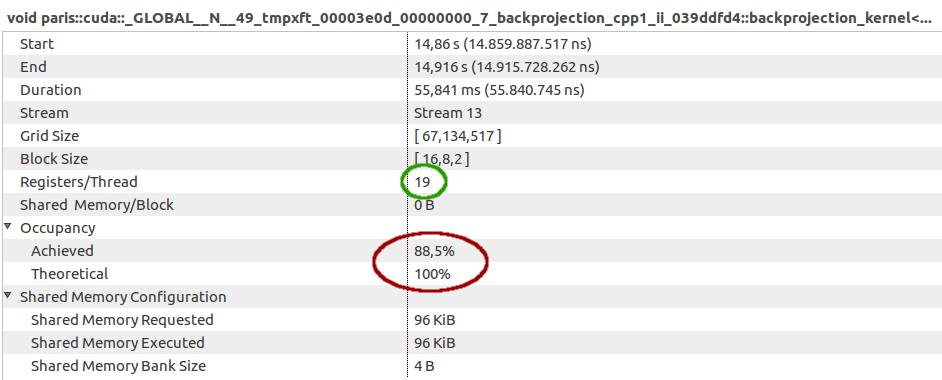
\includegraphics[width=\linewidth]{img/kernel_properties}
    \caption{Eigenschaften des Rückprojektionskernels}
    \label{fig:kernel_props}
\end{figure}

\begin{figure}
    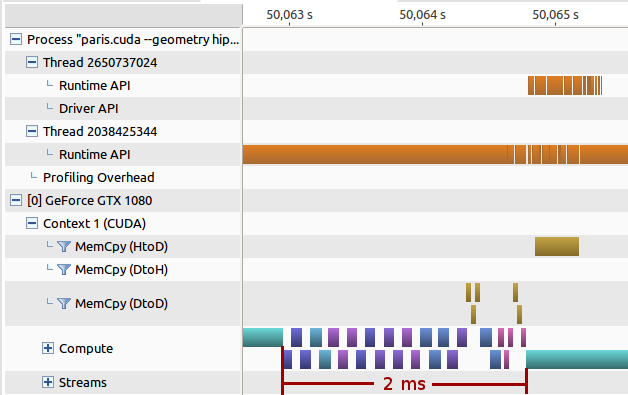
\includegraphics[width=\linewidth]{img/timeline_compute3}
    \caption{Zeit zwischen zwei Rückprojektionen}
    \label{fig:kernel_wait}
\end{figure}

\subsection{Laufzeitverhalten}

Die parallele Berechnung verschiedener Teile des Volumens durch den Einsatz mehrerer \gls{gpu}s war ebenfalls ein
Implementierungsziel. Die besondere Herausforderung bestand darin, sowohl mehrere \gls{gpu}s des gleichen Typs als auch
unterschiedliche \gls{gpu}s zu unterstützen.

Wie Abbildung~\ref{fig:kernel_multi_compute} zeigt, ist es gelungen, die Ausführung parallel auf mehreren \gls{gpu}s
durchzuführen. Der gewählte Ansatz zur Lastverteilung (siehe Abschnitt~\ref{}) führt jedoch bei unterschiedlich
leistungsstarken \gls{gpu}s dazu, dass die stärkere \gls{gpu} vor der schwächeren fertig ist und dann auf diese warten
muss, wie in Abbildung~\ref{fig:kernel_multi_bad} zu sehen ist.

In Abbildung~\ref{fig:laufzeit_gpus} ist das Laufzeitverhalten unterschiedlicher \gls{gpu}s dargestellt. Es ist klar
zu sehen, dass der gemeinsame Einsatz der Tesla K20c und der GTX 1080 in diesem Fall sogar zu einer längeren Laufzeit
führt, als der alleinige Einsatz der GTX 1080. Die statische Lastverteilung, wie sie in dieser Arbeit beschrieben ist,
sollte daher zukünftig auf heterogenen \gls{gpu}-Systemen durch andere Methoden abgelöst werden. Denkbar ist
beispielsweise der Einsatz von \textit{Machine-Learning}-Techniken, durch die die optimale Lastverteilung iterativ
ermittelt wird.

\begin{figure}
    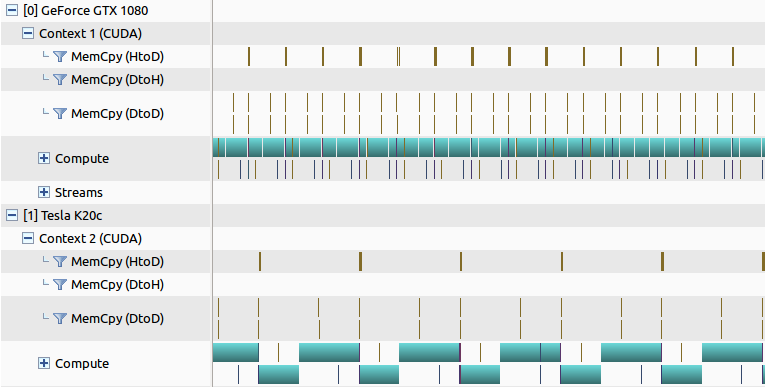
\includegraphics[width=\linewidth]{img/timeline_multi_compute}
    \caption{Parallele Ausführung auf zwei \gls{gpu}s}
    \label{fig:kernel_multi_compute}
\end{figure}

\begin{figure}
    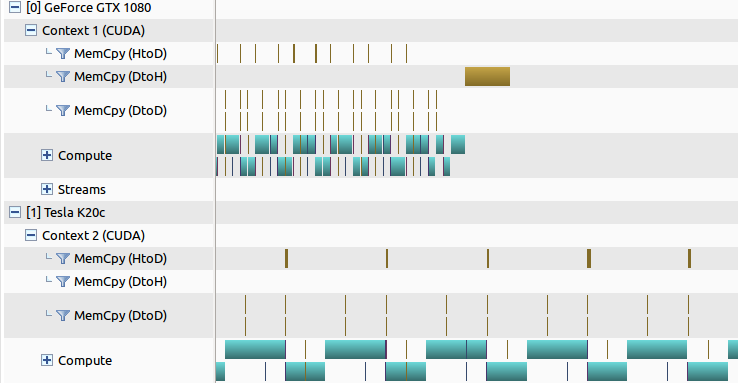
\includegraphics[width=\linewidth]{img/timeline_multi_bad}
    \caption{Der gewählte, statische Lastverteilungsansatz führt zu Wartezeiten}
    \label{fig:kernel_multi_bad}
\end{figure}

\begin{figure}
    \centering
    \begin{tikzpicture}
        \begin{axis}[width=\textwidth,
                     xlabel={Volumengröße [Voxel]},
                     symbolic x coords={133 x 133 x 129,267 x 267 x 258,535 x 535 x 516, 1070 x 1070 x 1033},
                     xtick=data,
                     ylabel={Laufzeit [s]},
                     legend pos=north west]

             \addplot table[x=Volumengroesse,y=GTX1080,col sep=comma] {data/mehreregpus.csv};
             \addplot table[x=Volumengroesse,y=K20c,col sep=comma] {data/mehreregpus.csv};
             \addplot table[x=Volumengroesse,y=GTX1080K20c,col sep=comma] {data/mehreregpus.csv};
             \legend{GTX 1080,Tesla K20c,GTX \& Tesla};
        \end{axis}
    \end{tikzpicture}
    \caption{Laufzeit mit mehreren \gls{gpu}s}
    \label{fig:laufzeit_gpus}
\end{figure}

\section{Vergleich mit der Literatur}

\chapter{Zusammenfassung und Ausblick}

Es wurde in dieser Arbeit eine mögliche Implementierung des \gls{fdk} auf dem Fundament der CUDA-Plattform vorgestellt.
Das Ziel, die Rückprojektion in sinnvoller Zeit zu berechnen, ist erreicht worden. Abhängig von der gewünschten Größe
des Volumens benötigt der Algorithmus auf moderner Hardware wenige Sekunden bis Minuten. Die Wartezeit zwischen zwei
Rückprojektionen konnte auf wenige Millisekunden reduziert werden. Insbesondere bei großen Volumen ist sie dadurch
vernachlässigbar gering, da sie, akkumuliert über die gesamte Laufzeit von einigen Minuten, lediglich wenige Sekunden
einnimmt. Bei der Rekonstruktion kleinerer Volumen fällt sie allerdings stärker ins Gewicht.

Es wurde ebenfalls erreicht, dass der Rückprojektions-\gls{kernel} die \gls{gpu} möglichst stark auslastet. Außerdem
gelang es, den Algorithmus so zu implementieren, dass er bei der Berechnung großer Volumen von mehreren \gls{gpu}s des
gleichen Typs beschleunigt wird. Die Rekonstruktion kleinerer Volumen profitiert allerdings nicht vom Einsatz mehrerer
Grafikkarten; eine einzelne \gls{gpu} war in allen Fällen schneller. Die Verwendung verschiedener \gls{gpu}s kann
außerdem dazu führen, dass der Algorithmus langsamer ausgeführt wird, als wenn man nur die leistungsstärkere Grafikkarte
verwendet hätte.

Die Verwendung von CUDA hat sich für die Parallelisierung des \gls{fdk} als vorteilhaft erwiesen. Durch die massiv
datenparallele Philosophie eignet sich CUDA gut für die Berechnung unabhängiger \gls{voxel}. Aufgrund der
Spezialisierung der \gls{gpu}s auf grafische Operationen sind sie gut für den Einsatz in bildgebenden Messverfahren wie
der Computertomographie geeignet. Eine Hürde, die beachtet werden muss, bleibt allerdings der begrenzte Speicher,
besonders im Hinblick auf die von neuen und zukünftigen Computertomographieanlagen erzeugten Datenmengen.

Wie die Analyse gezeigt hat, ist die vorgestellte Implementierung noch nicht an allen Stellen optimal. Insbesondere ist
es bei kleinen Volumen nicht gelungen, die in der Literatur präsentierten Zeiten für die Rekonstruktion zu erreichen,
was vermutlich auf zu starken Host-Overhead zurückzuführen ist. Dieser Overhead steigt durch den Einsatz mehrerer
\gls{gpu}s sogar noch weiter an, sodass der nächste Optimierungsschritt des Programms darin bestehen muss, die
Operationen auf der \gls{host}-Seite zu optimieren.

Die Skalierung des \gls{fdk} über mehrere \gls{gpu}s ist insgesamt verbesserungswürdig. Die Tatsache, dass selbst bei
der Rekonstruktion großer Volumen der Einsatz zwei verschiedener \gls{gpu}s länger dauert als der alleinige Einsatz der
leistungsstärkeren Karte, zeigt deutlich die Limitierungen der verwendeten statischen Lastverteilung. Denkbar ist hier
eine vor der Rückprojektion stattfindende algorithmische Bestimmung der idealen Last pro \gls{gpu}, beispielsweise in
Abhängigkeit von der Taktfrequenz und dem verfügbaren Speicher der jeweiligen Grafikkarte. Auch der Einsatz von
\textit{Machine-Learning}-Techniken kann in Betracht gezogen werden.

Die gefilterte Rückprojektion könnte außerdem durch einige Ansätze aus der Literatur weiter verbessert werden. Bei
großen Volumen wäre die Ausnutzung der Symmetrien, wie sie von Zhao et al.\ vorgeschlagen wird, eine Möglichkeit zur
weiteren Geschwindigkeitssteigerung. Der Ansatz von Scherl et al.\, mit einem zweidimensionalen Kernel durch das Volumen
zu iterieren, könnte die Zahl der für die Rückprojektion benötigten Ressourcen reduzieren und so auf dem \gls{device}
die zur Rückprojektion parallele Ausführung der Wichtung und Filterung erlauben. Dadurch wäre es möglich, die Zeit
zwischen zwei Rückprojektionen weiter zu reduzieren.

Die vorgestellte Implementierung des \gls{fdk} berechnet die Rückprojektion für derzeit gängige Projektionsdatensätze
in wenigen Minuten. Aufgrund der Aufnahmegeschwindigkeit einer Computertomographieanlage ist es denkbar, die
generierten Projektionen in Echtzeit zu verarbeiten. Die für die Berechnung benötigte Zeit könnte so durch die Aufnahme
verdeckt werden, sodass am Ende der Aufnahme bereits ein rekonstruiertes Volumen vorliegt. Dabei wäre es möglich bzw.\
für die Echtzeitrekonstruktion notwendig, vor der Wichtung und der Filterung der Projektionen zusätzliche
Vorverarbeitungsschritte in den Algorithmus zu integrieren, wie etwa eine Korrektur defekter Pixel oder eine
automatische Berücksichtigung des Detektor-Offsets.

Das im Rahmen dieser Arbeit am Helmholtz-Zentrum Dresden-Rossendorf entstandene Programm wurde unter eine freie Lizenz
gestellt. Der Quelltext ist im Internet unter der nachstehenden Adresse verfügbar:
\url{https://www.github.com/HZDR-FWDF/PARIS}


\end{document}
